\documentclass[10pt,twocolumn]{IEEEtran}

% Packages
\usepackage{algorithm}
\usepackage{algorithmic}
\usepackage{amsmath}
\usepackage{amssymb}
\usepackage{xcolor}
\usepackage{hyperref}
\usepackage{graphicx}
\usepackage{subfigure}
\usepackage{cite}
\usepackage{url}
\usepackage{balance}
\usepackage{booktabs}
\usepackage[justification=centering]{caption}

% Better spacing for IEEE format
\IEEEoverridecommandlockouts

% Graphics path
\graphicspath{{graphs/}}

% Custom commands for consistent formatting
\newcommand{\ie}{\textit{i.e.}}
\newcommand{\eg}{\textit{e.g.}}
\newcommand{\etal}{\textit{et al.}}

\begin{document}

\title{\large\textbf{DRAFT REPORT}\\[0.5em]\Large\textbf{Building World Models for Reinforcement Learning\\with Spectral Transform Units}}

\author{
\begin{tabular}[t]{c}
Shivam Kak\\
Princeton University\\
Department of Computer Science\\
\texttt{sk3686@princeton.edu}
\end{tabular}
\hspace{1.5cm}
\begin{tabular}[t]{c}
Elad Hazan (Advisor)\\
Princeton University\\
Department of Computer Science\\
\texttt{ehazan@princeton.edu}
\end{tabular}
}

\maketitle

\begin{abstract}
Reinforcement learning agents often suffer from sample inefficiency when learning complex tasks through trial and error. World models offer a solution by enabling agents to simulate future outcomes and practice in imagined rollouts. This thesis explores the use of Spectral Transform Units (STUs) as a core architecture for world models in discrete control environments, specifically within the EfficientZero V2 framework on Atari games. Through online experiments, we first evaluate various architectural modifications incorporating STUs into the value, policy, and dynamics networks. We then develop an offline dynamics training methodology that isolates the dynamics function while keeping the representation network fixed. Our key finding is that Spatial STU -- which applies spectral filtering across spatial positions of the latent state -- produces dynamics functions with dramatically improved long-horizon autoregressive stability compared to the baseline, Mamba, and self-attention alternatives. This is true even though all architectures seen during experimentation are trained only with single-step loss. On both Atari Pong and Asterix, the Spatial STU dynamics function maintains bounded prediction error over 50-step rollouts while the baseline diverges catastrophically after approximately 10 steps. We provide analysis suggesting that spectral filtering acts as a smoothness prior that suppresses high-frequency error modes at each step. However, we also claim that this long-horizon stability may not translate to improved online Atari performance, as the baseline dynamics function is sufficient for the short rollout lengths (5--10 steps) used in practice. Longer rollouts, such as the 50-step rollout used in offline experimentation, become computationally expensive online and may be more useful in domains other than Atari that strictly require longer planning horizons.
\end{abstract}

\begin{IEEEkeywords}
Reinforcement Learning, World Models, Spectral Transform Units, Spectral Filtering, Dynamical Systems, EfficientZero, Atari
\end{IEEEkeywords}

\section{Introduction}
\label{sec:introduction}

\IEEEPARstart{R}{einforcement} learning (RL) agents must learn to make decisions in complex environments by trial and error, which can be highly sample-inefficient. World models~\cite{ha2018world} offer a promising solution by allowing agents to simulate future outcomes and practice in imagined rollouts before taking real actions. However, learning accurate world models for control tasks remains challenging, particularly for long-horizon predictions where small errors compound over time.

This work is motivated by the observation that prediction errors in neural network-based world models tend to compound rapidly during autoregressive rollouts, limiting their utility for long-horizon planning. Improved world models could dramatically reduce the sample complexity of RL algorithms, making them more practical for real-world applications like robotics, autonomous systems, and control problems where data collection is expensive or risky.

The goal of this project is to develop and evaluate Spectral Transform Units (STUs)~\cite{agarwal2023spectral} as a core architecture for world models in discrete control reinforcement learning environments. We integrate STUs into the EfficientZero V2 (EZV2) algorithm~\cite{wang2024efficientzero} and evaluate their effectiveness on Atari environments.

Our work makes two primary contributions:

\begin{enumerate}
    \item \textbf{Spatial STU stabilizes long-horizon dynamics prediction.} We show that applying spectral filtering as a spatial mixer over the latent state grid produces dynamics functions that are inherently stable over long autoregressive rollouts (tested up to 50 steps), even when trained with only single-step loss. This may be because spectral filtering over the $6 \times 6$ spatial grid acts as a regularizer on the latent state structure at each step, preventing error accumulation. This effect is significantly stronger than comparable modifications using Mamba~\cite{gu2024mamba} or self-attention~\cite{vaswani2017attention}. This result is achieved with ${\sim}30\%$ fewer parameters than the baseline EZV2 dynamics function.

    \item \textbf{Long-horizon stability likely will not translate to improved online Atari performance.} Despite the strong offline results, we find that the baseline EZV2 dynamics function is sufficient for the short unroll lengths (5--10 steps) used during online training. Increasing the number of recurrent unroll steps to leverage STU's advantage is computationally prohibitive and does not correlate with improved policy or value loss. This suggests that STU's inductive bias is useful for long-horizon prediction stability, but long-horizon prediction stability might not be useful for solving online Atari efficiently.
\end{enumerate}

\section{Background and Related Work}
\label{sec:background}

\subsection{World Models for Reinforcement Learning}

World models learn a predictive model of the environment that an RL agent can use for planning. Early work by Ha and Schmidhuber~\cite{ha2018world} demonstrated that agents can learn compact representations of their environment and use them for decision-making. More recently, DreamerV3~\cite{hafner2023dreamerv3} showed that world models can master diverse domains. The MuZero family of algorithms~\cite{schrittwieser2020mastering, wang2024efficientzero} learns world models in a latent space and performs planning using Monte Carlo Tree Search (MCTS).

\subsection{Limitations of Existing World Model Architectures}

Existing world model architectures face several limitations. Recurrent neural networks suffer from vanishing gradients and struggle with long sequences. Transformer-based models, while powerful, require substantial computational resources and may not capture the underlying dynamical structure of physical systems efficiently. Most critically, prediction errors in neural network-based world models tend to compound rapidly over time, limiting their utility for long-horizon planning.

\subsection{State Space Models}

Structured State Space models (S4)~\cite{gu2022efficiently} and their variants have emerged as efficient alternatives for sequence modeling. Mamba~\cite{gu2024mamba} extends this line of work with selective state spaces that achieve linear-time sequence modeling. STUs~\cite{agarwal2023spectral} offer a fundamentally different approach rooted in spectral methods for learning dynamical systems, originally developed for linear dynamical systems~\cite{hazan2017learning} and recently extended to universal nonlinear dynamics.

\subsection{EfficientZero V2 Algorithm}

The EfficientZero V2 algorithm~\cite{wang2024efficientzero} learns a predictive model in a latent space and then performs planning over actions using this model. The components consist of:

\begin{itemize}
    \item \textbf{Representation Function}: $H: s_t = H(o_t)$  --  learns a compact state representation of the input observation $o_t$
    \item \textbf{Dynamic Function}: $G: \hat{s}_{t+1}, r_t = G(s_t, a_t)$  --  predicts the next state $\hat{s}_{t+1}$ and the reward $r_t$
    \item \textbf{Policy Function}: $P: p_t = P(s_t)$  --  outputs the current policy $p_t$
    \item \textbf{Value Function}: $V: v_t = V(s_t)$  --  provides the value estimation $v_t$ at the current state
\end{itemize}

All components are implemented as neural networks. The action embedding block $A$ encodes the action $a_t$ as a latent vector within the dynamic function. The latent state $s_t$ has shape $[B, C, 6, 6]$ where $B$ is the batch size and $C = 64$ is the number of channels.

\subsection{Spectral Filtering Theory}

A Spectral Transform Unit (STU) is a sequence-to-sequence neural network layer~\cite{agarwal2023spectral}. Given an input sequence $\{u_1, \ldots, u_L\} \in \mathbb{R}^{d_{in}}$, it produces an output sequence $\{y_1, \ldots, y_L\} \in \mathbb{R}^{d_{out}}$. A single layer of STU is parameterized by a number $K$ denoting the number of eigenfactors, and matrices $M^{\phi+}_1, \ldots, M^{\phi+}_K$, $M^{\phi-}_1, \ldots, M^{\phi-}_K \in \mathbb{R}^{d_{out} \times d_{in}}$, and $M^u_1, M^u_2, M^u_3 \in \mathbb{R}^{d_{out} \times d_{in}}$.

The Hankel matrix $Z \in \mathbb{R}^{L \times L}$ whose entries are given by:
\begin{equation}
Z[i, j] \triangleq \frac{2}{(i + j)^3 - (i + j)}
\end{equation}

Let $\{(\sigma_j \in \mathbb{R}, \phi_j \in \mathbb{R}^L)\}^L_{j=1}$ be the eigenvalue-eigenvector pairs of $Z$ ordered to satisfy $\sigma_1 \geq \sigma_2 \geq \ldots \geq \sigma_d$. The STU computes the output by convolving the input with the top-$K$ eigenvectors of $Z$. These eigenvectors form an ordered basis from low-frequency to high-frequency patterns: when $K$ is small, it is likely that the STU projects through a basis that emphasizes smooth, slowly-varying structure and suppresses high-frequency components.

\section{Approach and Methodology}
\label{sec:approach}

Our approach proceeds in two phases: online integration of STUs into the full EZV2 training loop (Phase 1), and offline dynamics training that isolates the dynamics function while keeping the latent space generated by the representation network fixed (Phase 2).

\subsection{Phase 1: Online STU Integration}

We integrate STU layers into the EZV2 architecture at various points:

\begin{enumerate}
    \item \textbf{Value/Policy Networks}: Adding STU layers to the value and policy prediction heads
    \item \textbf{Dynamics Network}: Incorporating STU layers in the dynamics function with residual connections
    \item \textbf{History Tracking}: Implementing a history buffer to provide real sequences of input states to STU layers
\end{enumerate}

We evaluate these modifications on the Atari Pong environment, using training loss, policy loss, and evaluation scores as our primary metrics. Each experiment runs for approximately 100,000 training steps (${\sim}$15 hours on an A100 GPU).

\subsection{Phase 2: Offline Dynamics Training}
\label{sec:offline}

To address the computational cost of full online training runs and the lack of a direct dynamics loss in EZV2, we developed an offline training methodology:

\begin{enumerate}
    \item \textbf{Expert Data Collection}: Train a baseline EZV2 model for 100K--110K steps to obtain an ``expert'' checkpoint. Using this checkpoint's frozen representation network, collect a dataset of state transitions $(s_t, a_t, s_{t+1})$ in the latent space.
    \item \textbf{Offline Training}: Train only the dynamics function $G$ on single-step prediction loss:
    \begin{equation}
    \mathcal{L} = \text{MSE}(G(s_t, a_t), s_{t+1})
    \end{equation}
    \item \textbf{Multi-step Rollout Evaluation}: Evaluate the trained dynamics function by autoregressively generating predictions for $T$ steps and measuring MSE at each step against ground-truth states from the dataset. We set $T = 50$ for all experiments.
\end{enumerate}

This methodology provides two key advantages: (1) dramatically faster iteration (${\sim}$4 minutes per training run vs.\ ${\sim}$15 hours for full online training), and (2) a direct metric for dynamics prediction quality through multi-step rollout MSE. We published the collected datasets on HuggingFace\footnote{\url{https://huggingface.co/datasets/Shivamkak/STUZero-Atari-Dynamics}} for reproducibility. The code for all experiments is available on GitHub\footnote{\url{https://github.com/Shivamkak19/STUZero/}}.

\subsection{Architecture Variants}
\label{sec:arch-variants}

We evaluate the following dynamics function architectures, all structured as modifications to the baseline EZV2 dynamics network. Each variant adds a residual block after the initial convolution and batch normalization:

\textbf{Baseline}: The standard EZV2 dynamics network consisting of a convolution, batch normalization, residual connection, and residual blocks.

\textbf{Spatial STU}: After the baseline convolution, batch normalization, and residual connection with the input state, the intermediate representation $x \in \mathbb{R}^{B \times C \times 6 \times 6}$ is passed through a MiniSTU block as a spatial mixer. The representation is reshaped to $[B, 36, C]$, treating the $6 \times 6$ spatial positions as the sequence dimension:
\begin{equation}
x_{\text{new}} = \text{ReLU}(x + \text{MiniSTU}(x.\text{reshape}(B, 36, C)))
\end{equation}
The output is then passed through the residual blocks, as in the baseline.

\textbf{Temporal STU}: Maintains a history buffer of $N$ past states. For each spatial position, the $N$ timesteps are processed by a MiniSTU, extracting temporal dependencies across the history.

\textbf{Spatial-Temporal STU}: Applies both spatial and temporal STU blocks in sequence with residual connections.

\textbf{Spatial Mamba}: Same residual structure as Spatial STU, but replaces the MiniSTU block with a Mamba SSM layer~\cite{gu2024mamba}.

\textbf{Temporal Mamba}: Same structure as Temporal STU, but uses Mamba over the time dimension.

\textbf{Spatial Attention}: Same residual structure, but replaces the STU block with multi-head self-attention~\cite{vaswani2017attention} over spatial positions.

\textbf{Temporal Attention}: Same structure as Temporal STU, but uses multi-head self-attention over the time dimension.

\section{Experiments: Phase 1  --  Online Training}
\label{sec:online}

\subsection{Experiments 1--2: STU in Value and Policy Networks}

In the first experiment, we added a MiniSTU layer to the value prediction function within the ValuePolicy network.

\begin{figure*}[t]
\centering
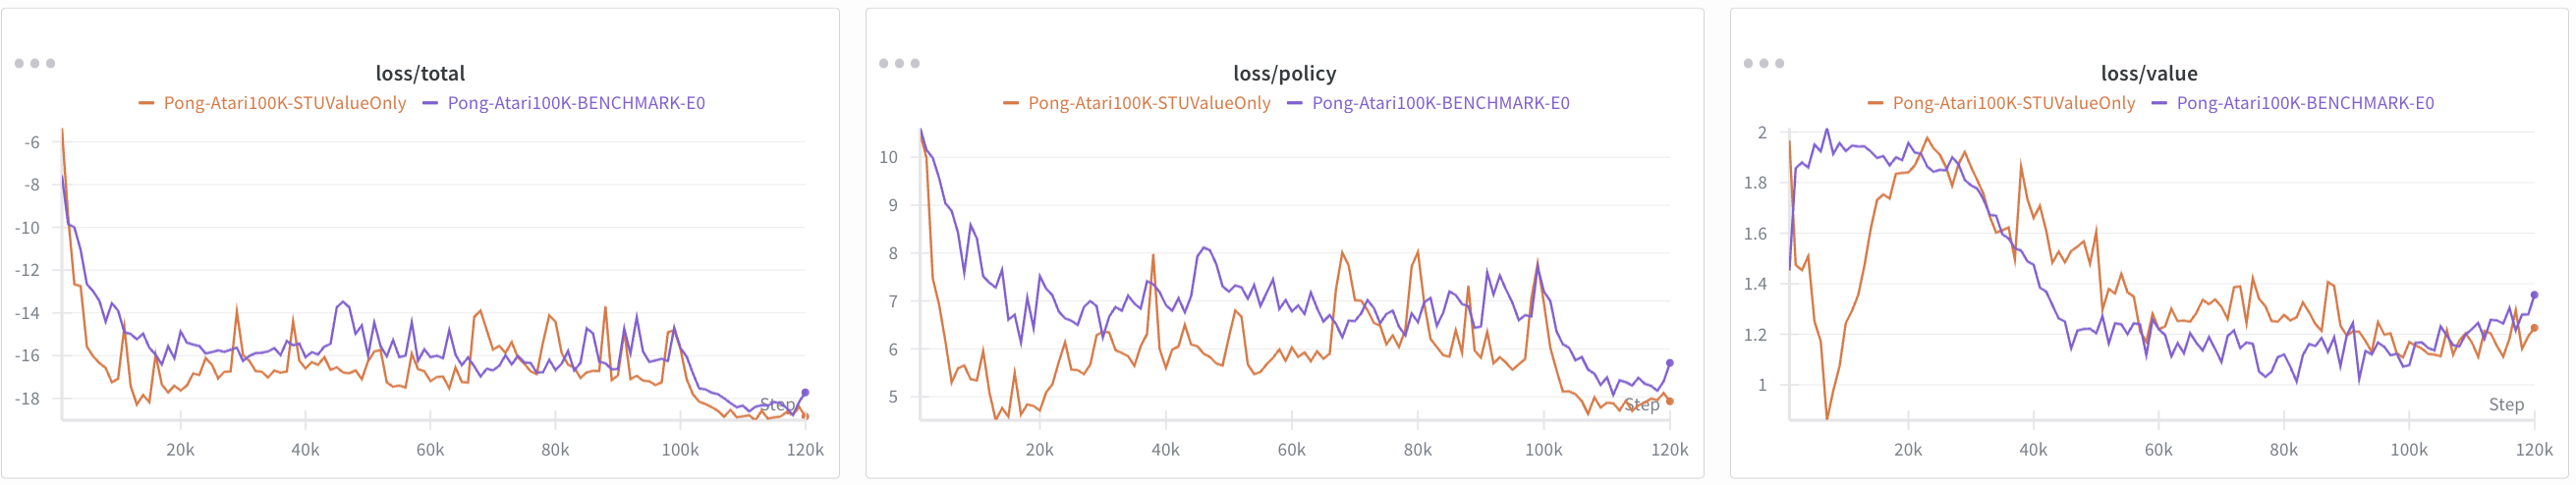
\includegraphics[width=0.9\textwidth]{EXP1_stu_value_only.png}
\caption{Experiment 1: STU added to value prediction only.}
\label{fig:exp1}
\end{figure*}

As shown in Figure~\ref{fig:exp1}, the STU version achieved a total loss of approximately $-18.2$ roughly 8.3$\times$ faster than the benchmark version (STU: 13,000 steps vs.\ benchmark: 108,000 steps). However, the STU version subsequently overcorrected, and the final evaluation score did not beat the benchmark.

\begin{figure*}[t]
\centering
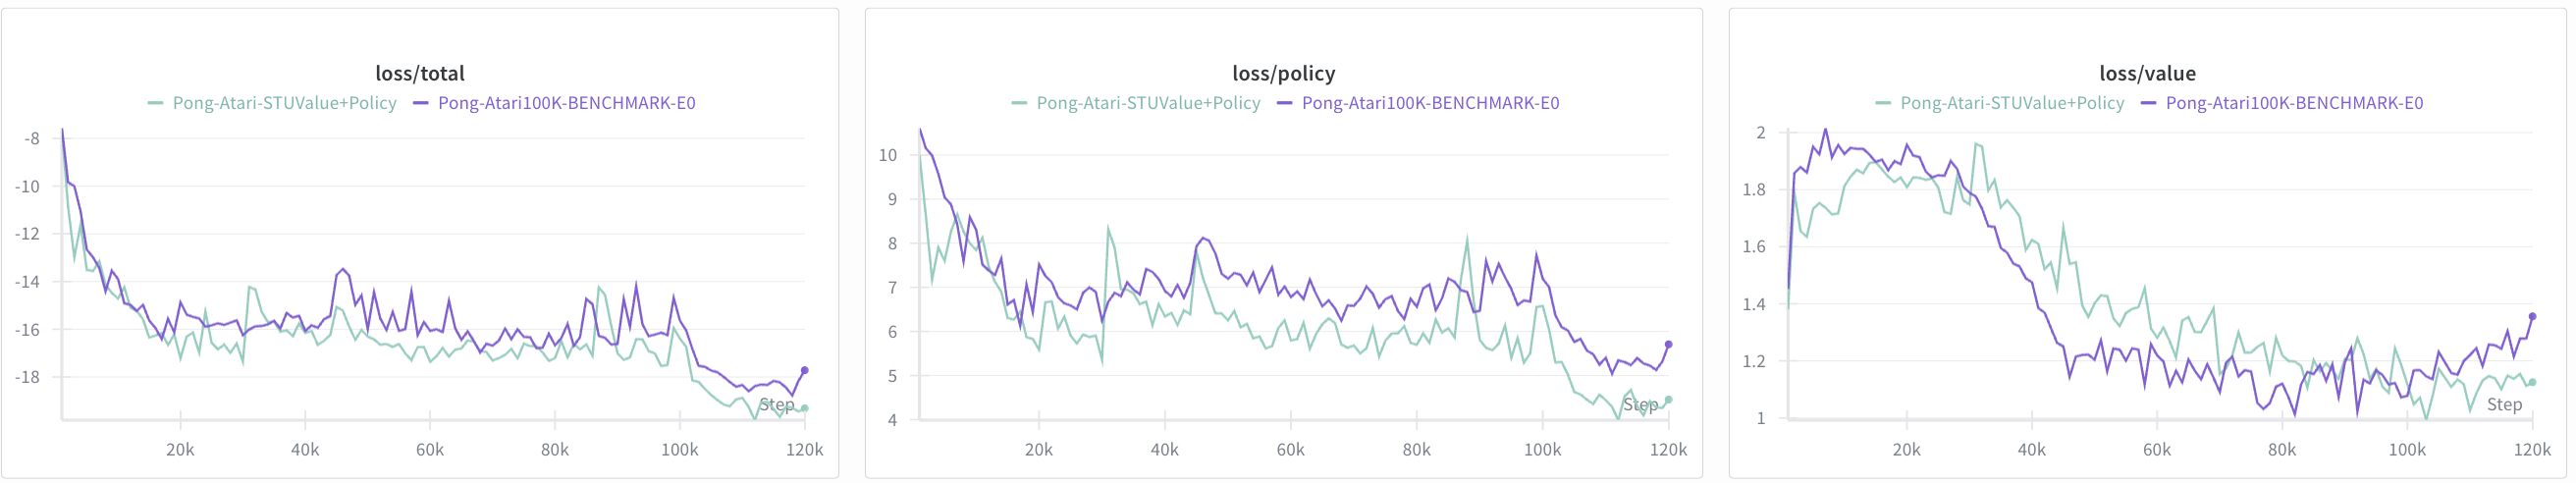
\includegraphics[width=0.9\textwidth]{EXP2_stu_value_policy.png}
\caption{Experiment 2: STU in value and policy prediction.}
\label{fig:exp2}
\end{figure*}

We extended the STU integration to both the value and policy prediction heads (Figure~\ref{fig:exp2}), which showed a similar pattern of rapid initial convergence followed by instability.

\subsection{Experiments 3--5: Hyperparameter Tuning}

To address the overfitting observed in Experiments 1 and 2, we conducted three hyperparameter tuning experiments (Figure~\ref{fig:exp3-5}):

\begin{figure*}[t]
\centering
\subfigure[Reduced learning rate (10$\times$ decrease)]{
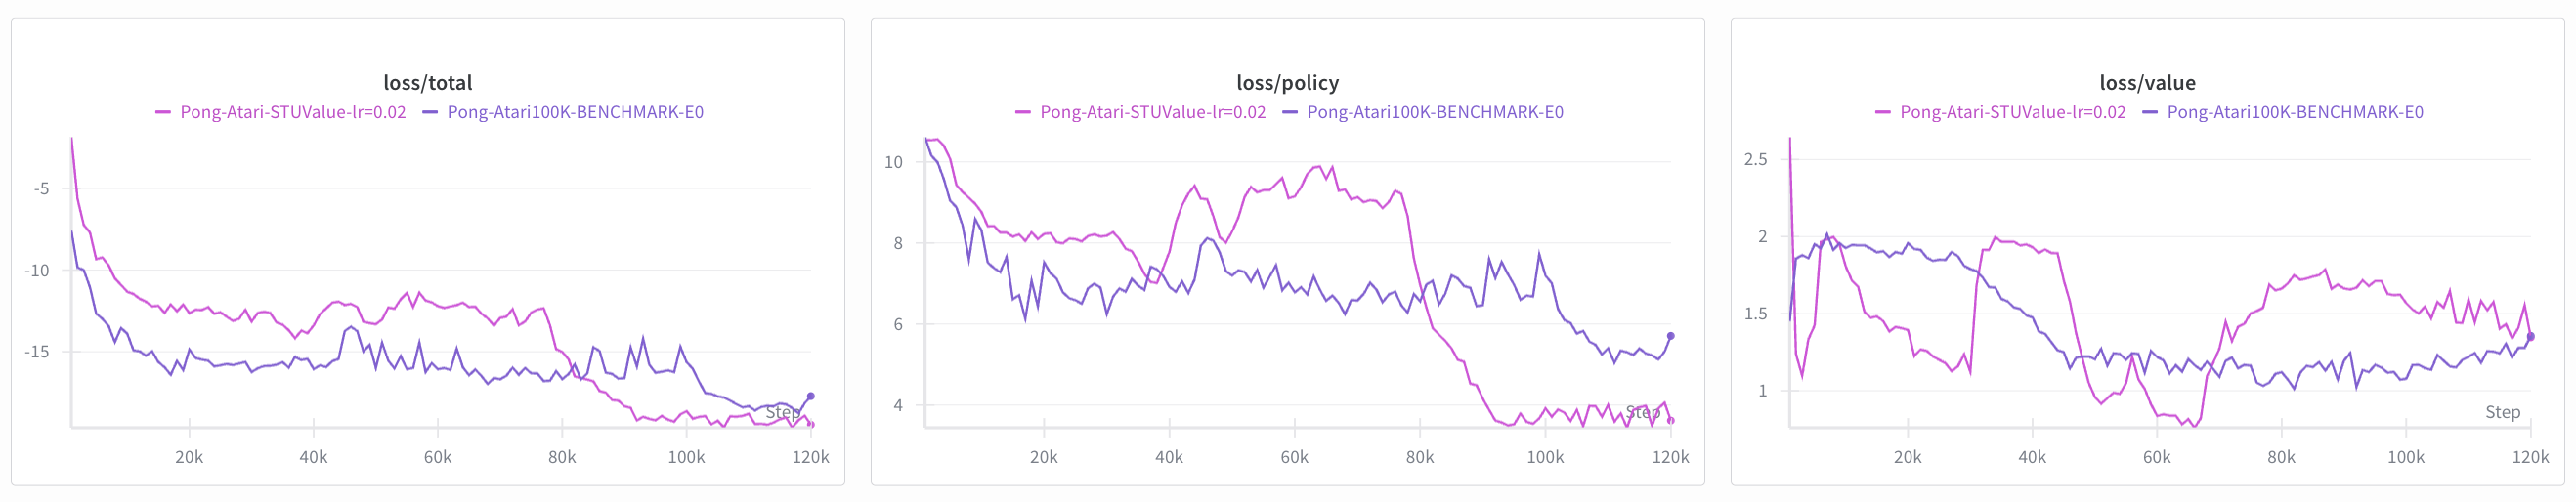
\includegraphics[width=0.7\textwidth]{EXP3_stu_value_lowLR.png}\label{fig:exp3}}

\subfigure[Increased weight decay (5$\times$ increase)]{
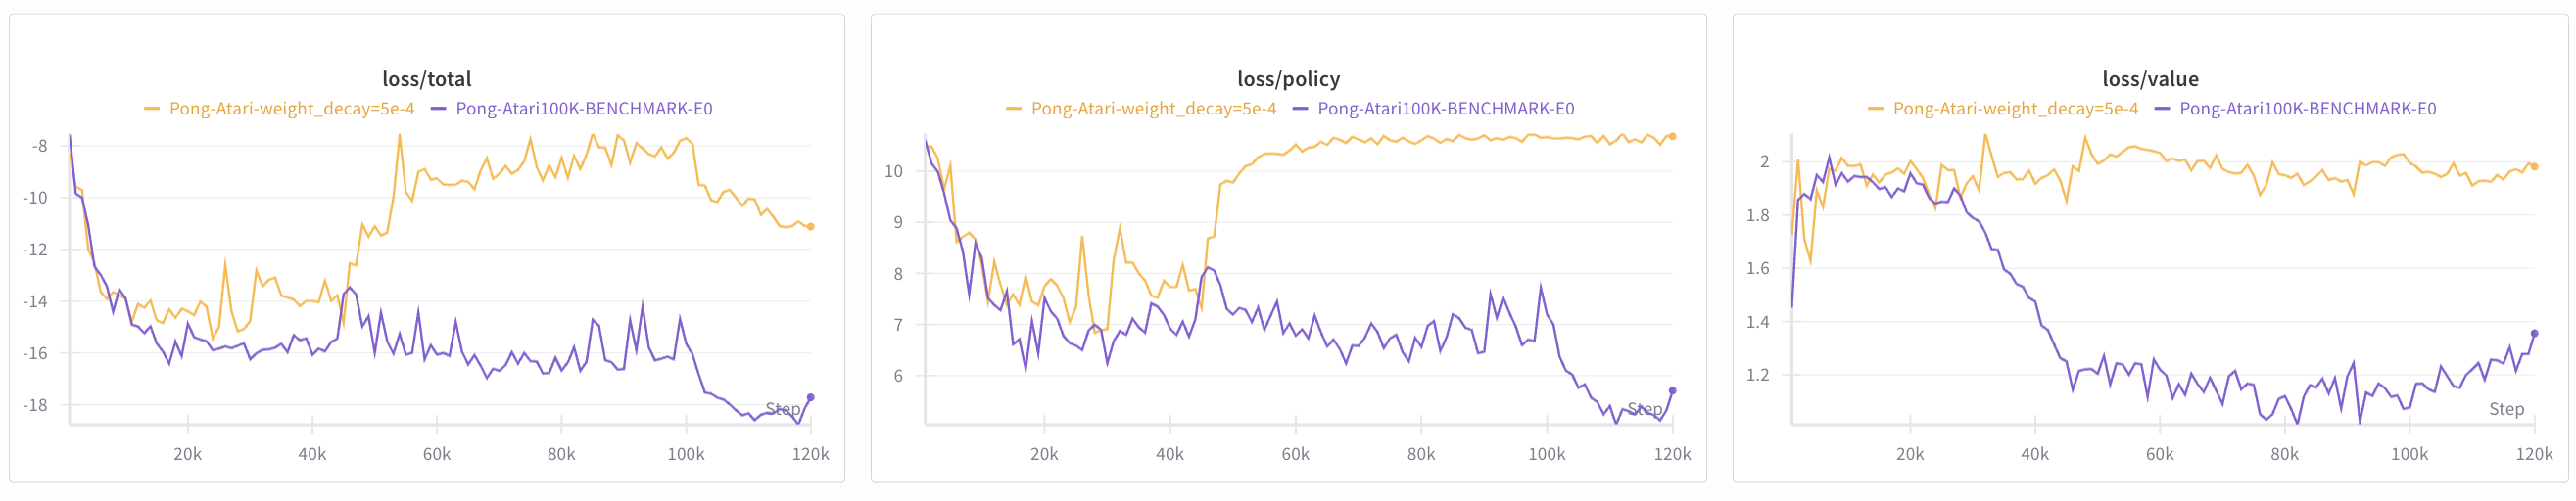
\includegraphics[width=0.7\textwidth]{EXP4_stu_value_highWD.png}\label{fig:exp4}}

\subfigure[Increased filters (8 $\to$ 16)]{
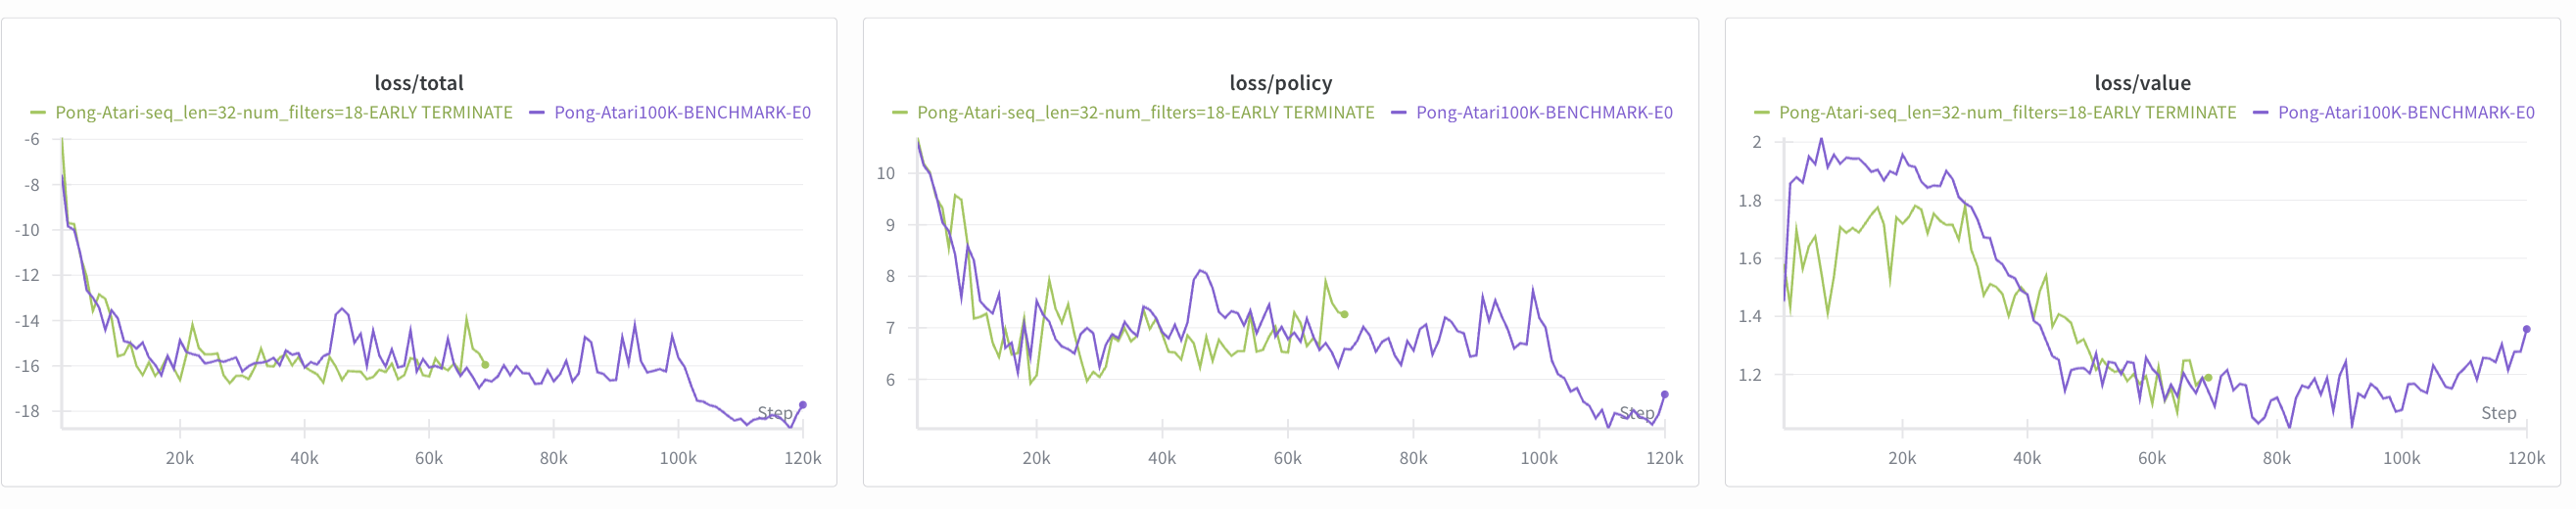
\includegraphics[width=0.7\textwidth]{EXP5_stu_value_morefilters.png}\label{fig:exp5}}
\caption{Experiments 3--5: Hyperparameter tuning attempts.}
\label{fig:exp3-5}
\end{figure*}

\begin{itemize}
    \item \textbf{Experiment 3} (Figure~\ref{fig:exp3}): Reduced learning rate by 10$\times$
    \item \textbf{Experiment 4} (Figure~\ref{fig:exp4}): Increased weight decay by 5$\times$
    \item \textbf{Experiment 5} (Figure~\ref{fig:exp5}): Increased filters from 8 to 16
\end{itemize}

None of these modifications resulted in performance exceeding the original baseline.

\subsection{Experiments 6--7: STU in Dynamics Network}

Given the limited success with value/policy modifications, we shifted focus to the dynamics network.

\begin{figure*}[t]
\centering
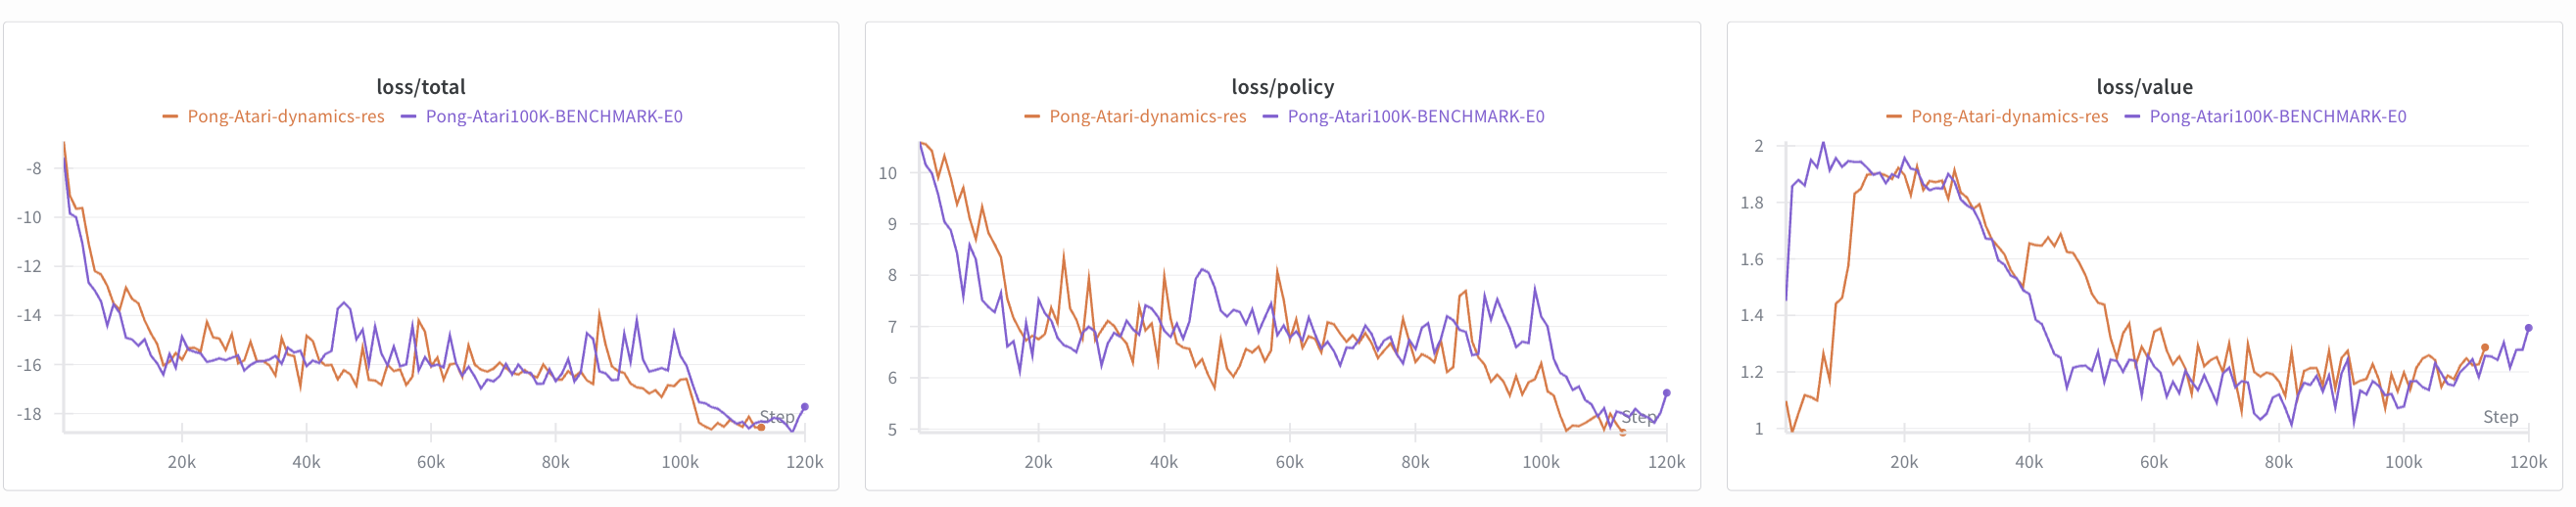
\includegraphics[width=0.9\textwidth]{EXP6_dynamics_residual.png}
\caption{Experiment 6: STU in dynamics network with residual connection.}
\label{fig:exp6}
\end{figure*}

\textbf{Experiment 6} (Figure~\ref{fig:exp6}): We added the Spatial STU block to the dynamics network, as described in Section~\ref{sec:arch-variants}.

\begin{figure*}[t]
\centering
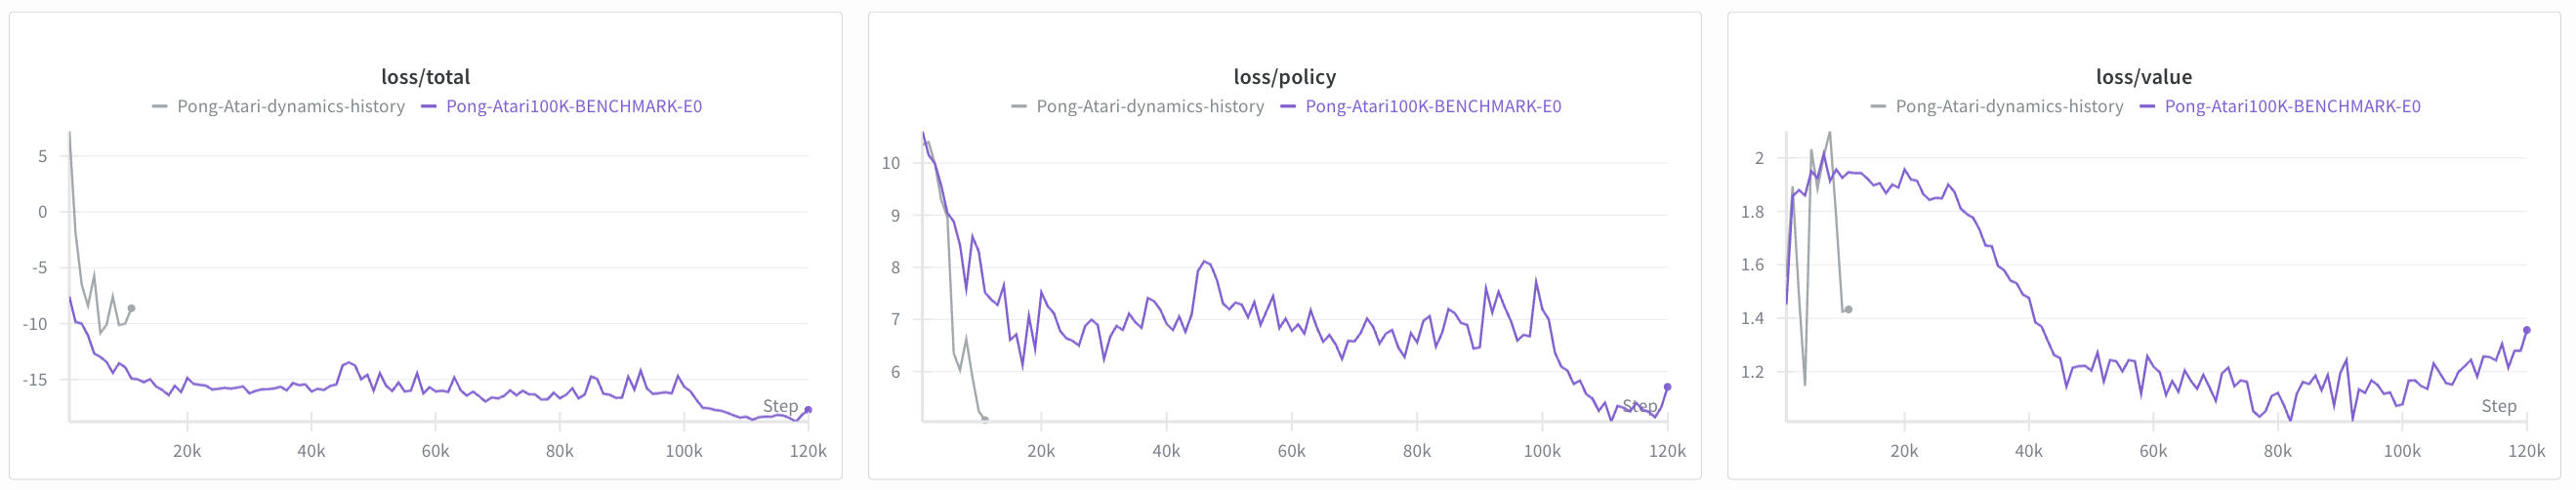
\includegraphics[width=0.9\textwidth]{EXP7_dynamics_history.png}
\caption{Experiment 7: STU with history buffer in dynamics network.}
\label{fig:exp7}
\end{figure*}

\textbf{Experiment 7} (Figure~\ref{fig:exp7}): We implemented a HistoryMiniSTU component that maintains a history buffer of input states. While this approach showed some changes in policy loss, total loss remained greater than the benchmark, and the training loop terminated early due to memory issues from the large input state buffer.

\subsection{Phase 1 Summary}

The online experiments revealed two key insights: (1) STU can accelerate initial convergence (Experiment 1), and (2) the EZV2 online training loop does not provide a direct dynamics loss, as the dynamics network is trained jointly with the representation network and ValuePolicy network. Training jointly makes it difficult to evaluate whether modifications to the dynamics network improve state transition predictions. These observations motivated the development of the offline training methodology described in Section~\ref{sec:offline}.

\section{Experiments: Phase 2  --  Offline Dynamics Training}
\label{sec:offline-results}

\subsection{Experimental Setup}

We trained expert baseline EZV2 models for Atari Pong (action space size 6) and Atari Asterix (action space size 9) for 100K and 110K steps respectively. These step counts correlate with the step at which the baseline model achieved maximum eval scores for each game. Using these checkpoints we collected datasets of 50 episodes, each containing latent state transitions. Training and evaluation were split 40/10 episodes. For Pong, this yielded approximately 70K training transitions and 17K evaluation transitions, with 345 rollout windows of length 50 from the evaluation set. For Asterix, this yielded approximately 148K training transitions and 37K evaluation transitions, with 739 rollout windows of length 50.

All dynamics function variants were trained for 80 epochs with MSE loss on single-step prediction. Rollout evaluation was performed every 5 epochs.

\subsection{Experiment 8: Spatial STU vs.\ Baseline on Pong}
\label{sec:exp8}

\begin{figure*}[t]
\centering
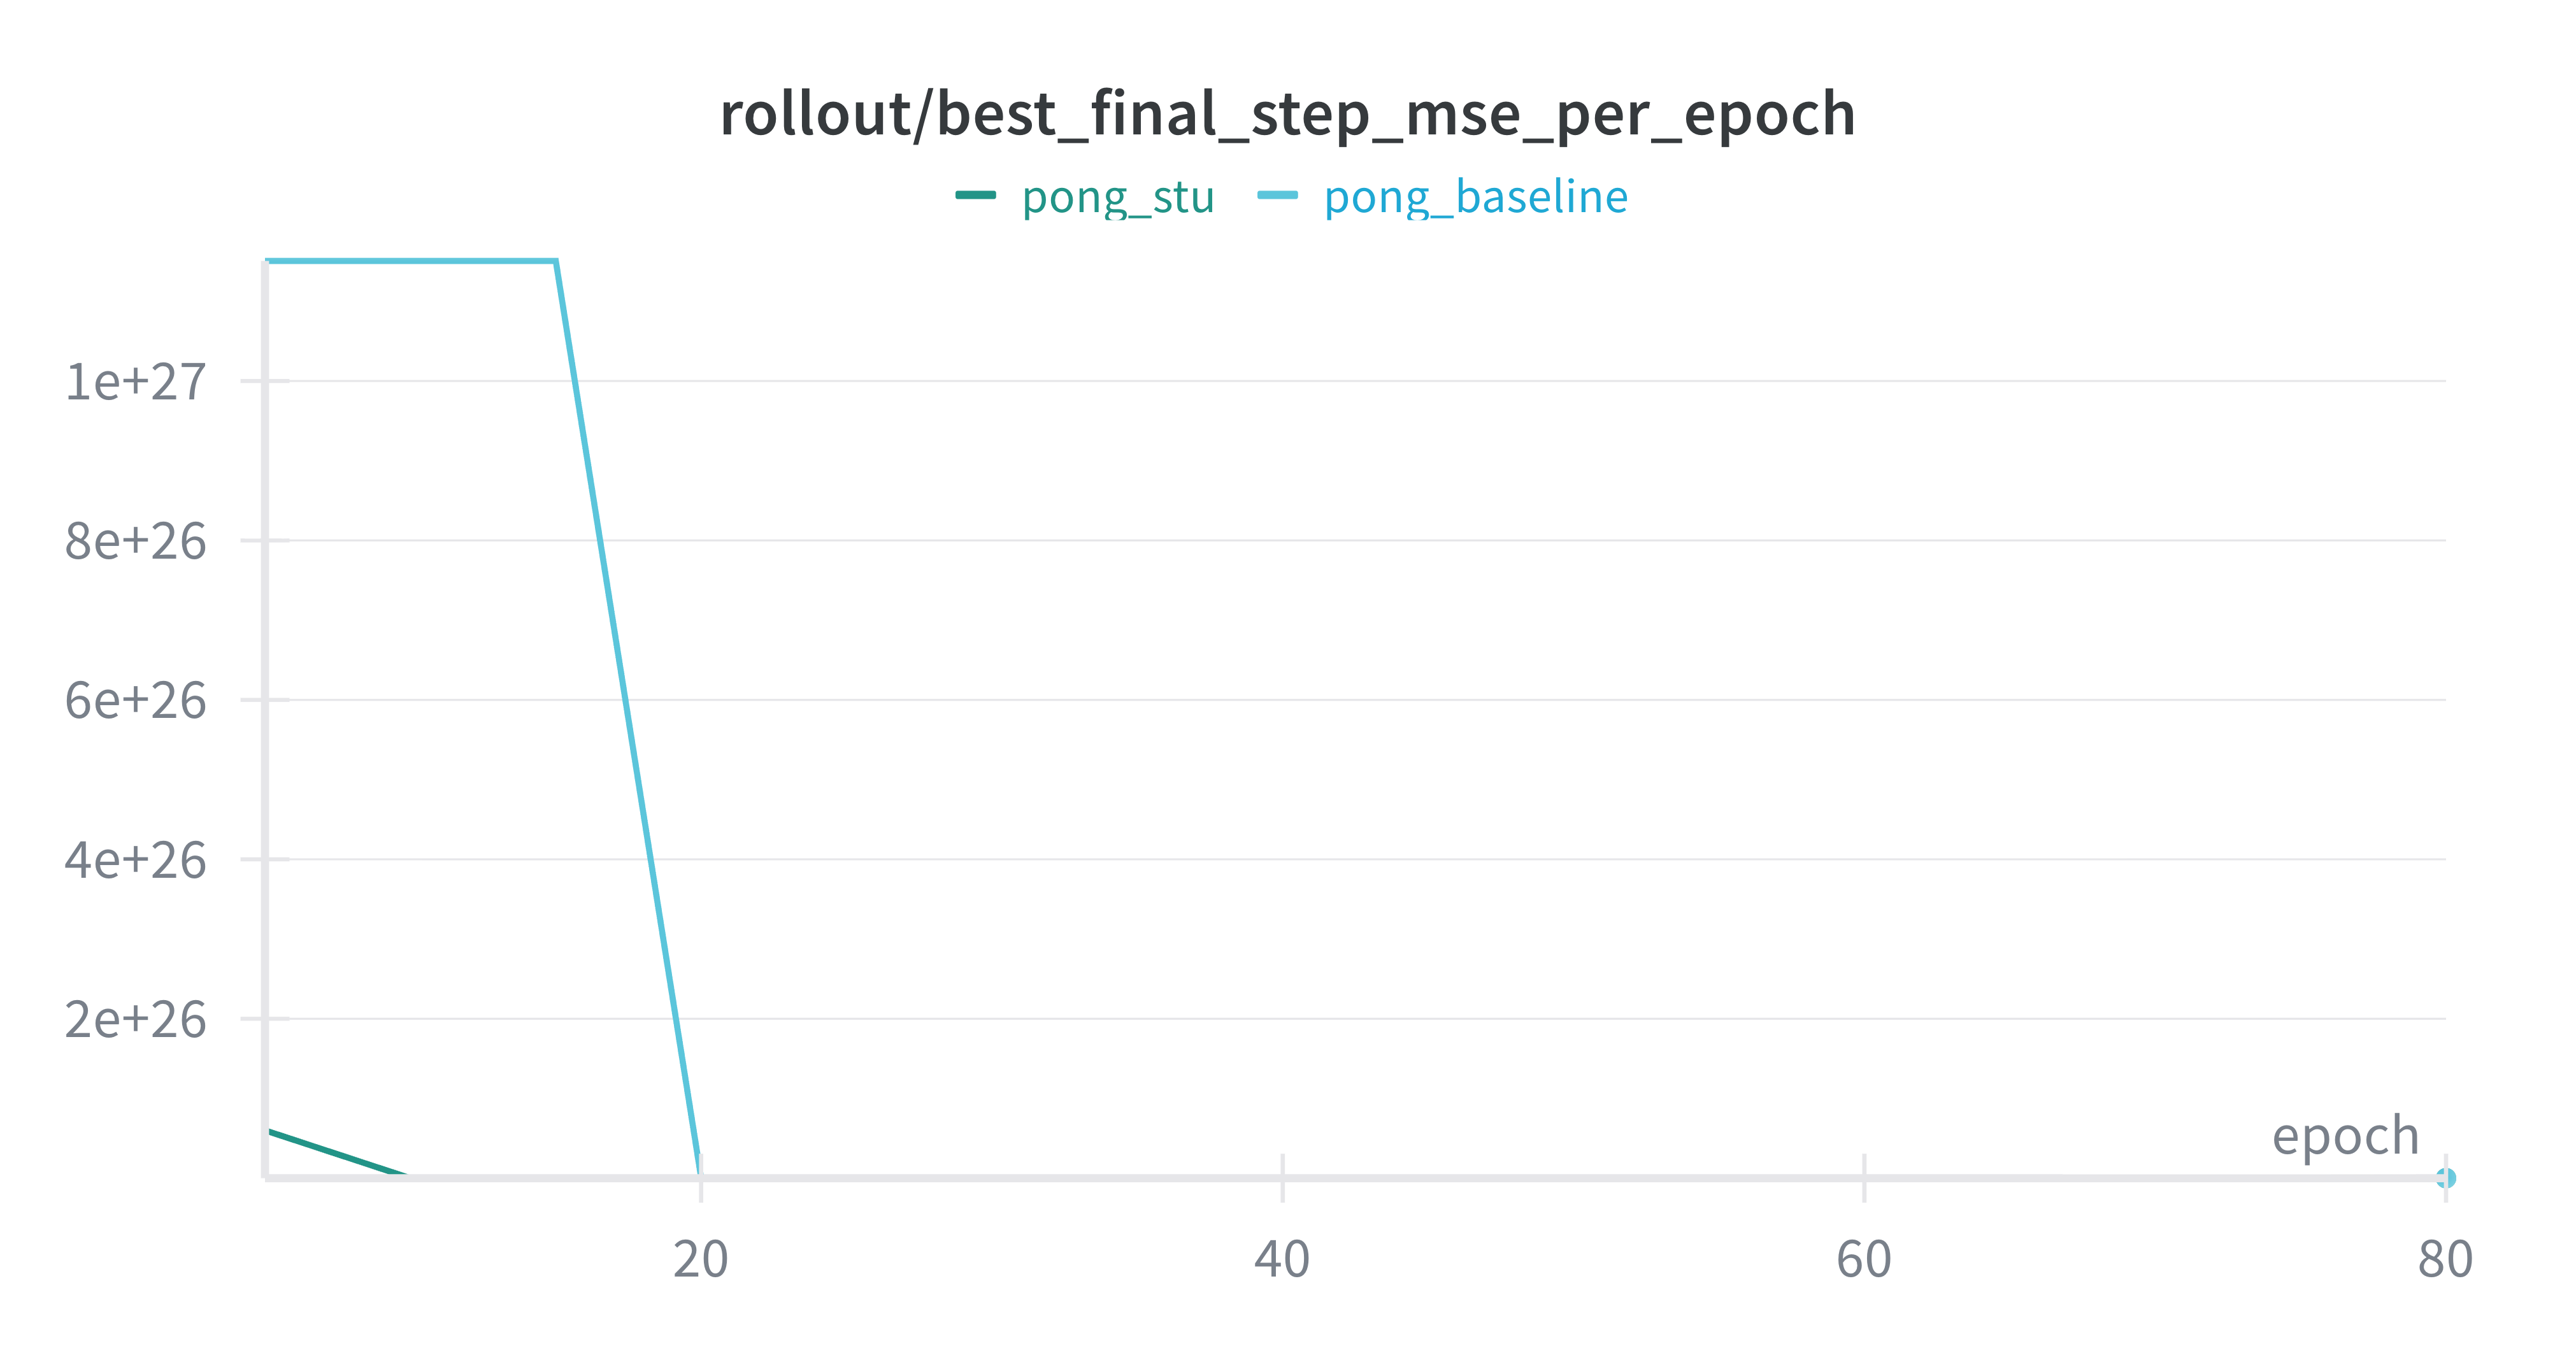
\includegraphics[width=0.9\textwidth]{EXP8_best_final_step_mse_pong.png}
\caption{Experiment 8: Best final step MSE (step 50 of rollout) over training epochs for Pong. The Spatial STU dynamics function converges to a bounded MSE ${\sim}0.82$, while the baseline remains at ${\sim}2.96 \times 10^{15}$.}
\label{fig:exp8}
\end{figure*}

The most significant result of this thesis is shown in Figure~\ref{fig:exp8}. The Spatial STU dynamics function (with $K=2$ filters, 1 residual block, 137,760 trainable parameters) achieves a best final-step MSE at step 50 of approximately $0.82$, while the baseline dynamics function (with 2 residual blocks, 195,360 trainable parameters) achieves a best final-step MSE of approximately $2.96 \times 10^{15}$.

Table~\ref{tab:pong} shows the best MSE achieved at selected rollout steps across all training epochs.

\begin{table}[t]
\centering
\caption{Best multi-step rollout MSE per step: Baseline vs.\ Spatial STU on Pong.}
\label{tab:pong}
\begin{tabular}{@{}crrl@{}}
\toprule
Step & Baseline & STU & Ratio \\
\midrule
1  & 0.0013 & 0.0015 & Baseline 1.1$\times$ better \\
5  & 0.017  & 0.004  & STU 4.1$\times$ better \\
10 & 0.53   & 0.007  & STU 79$\times$ better \\
20 & $2.8 \times 10^3$ & 0.022 & STU ${\sim}1.3 \times 10^5$ $\times$ better \\
30 & $2.8 \times 10^7$ & 0.14 & STU ${\sim}2 \times 10^8$ $\times$ better \\
40 & $4.0 \times 10^{11}$ & 0.21 & STU ${\sim}1.9 \times 10^{12}$ $\times$ better \\
50 & $2.96 \times 10^{15}$ & 0.82 & STU ${\sim}3.6 \times 10^{15}$ $\times$ better \\
\bottomrule
\end{tabular}
\end{table}

Critically, both models achieve comparable single-step prediction accuracy (MSE ${\sim}0.001$ after training), meaning the difference manifests only during autoregressive rollout. The baseline's error begins to compound catastrophically after approximately 10 steps, while the Spatial STU dynamics function maintains bounded error through all 50 steps. The Spatial STU model achieves this with approximately 30\% fewer parameters than the baseline.

We also tested configurations with varying numbers of residual blocks and filters. The baseline performed better with more blocks (larger network), while the STU variant performed worse with additional blocks. With $K=4$ filters, STU performance also degraded, consistent with the hypothesis that retaining higher-frequency spectral modes reintroduces instability.

\subsection{Experiment 9: Spatial STU vs.\ Baseline on Asterix}

\begin{figure*}[t]
\centering
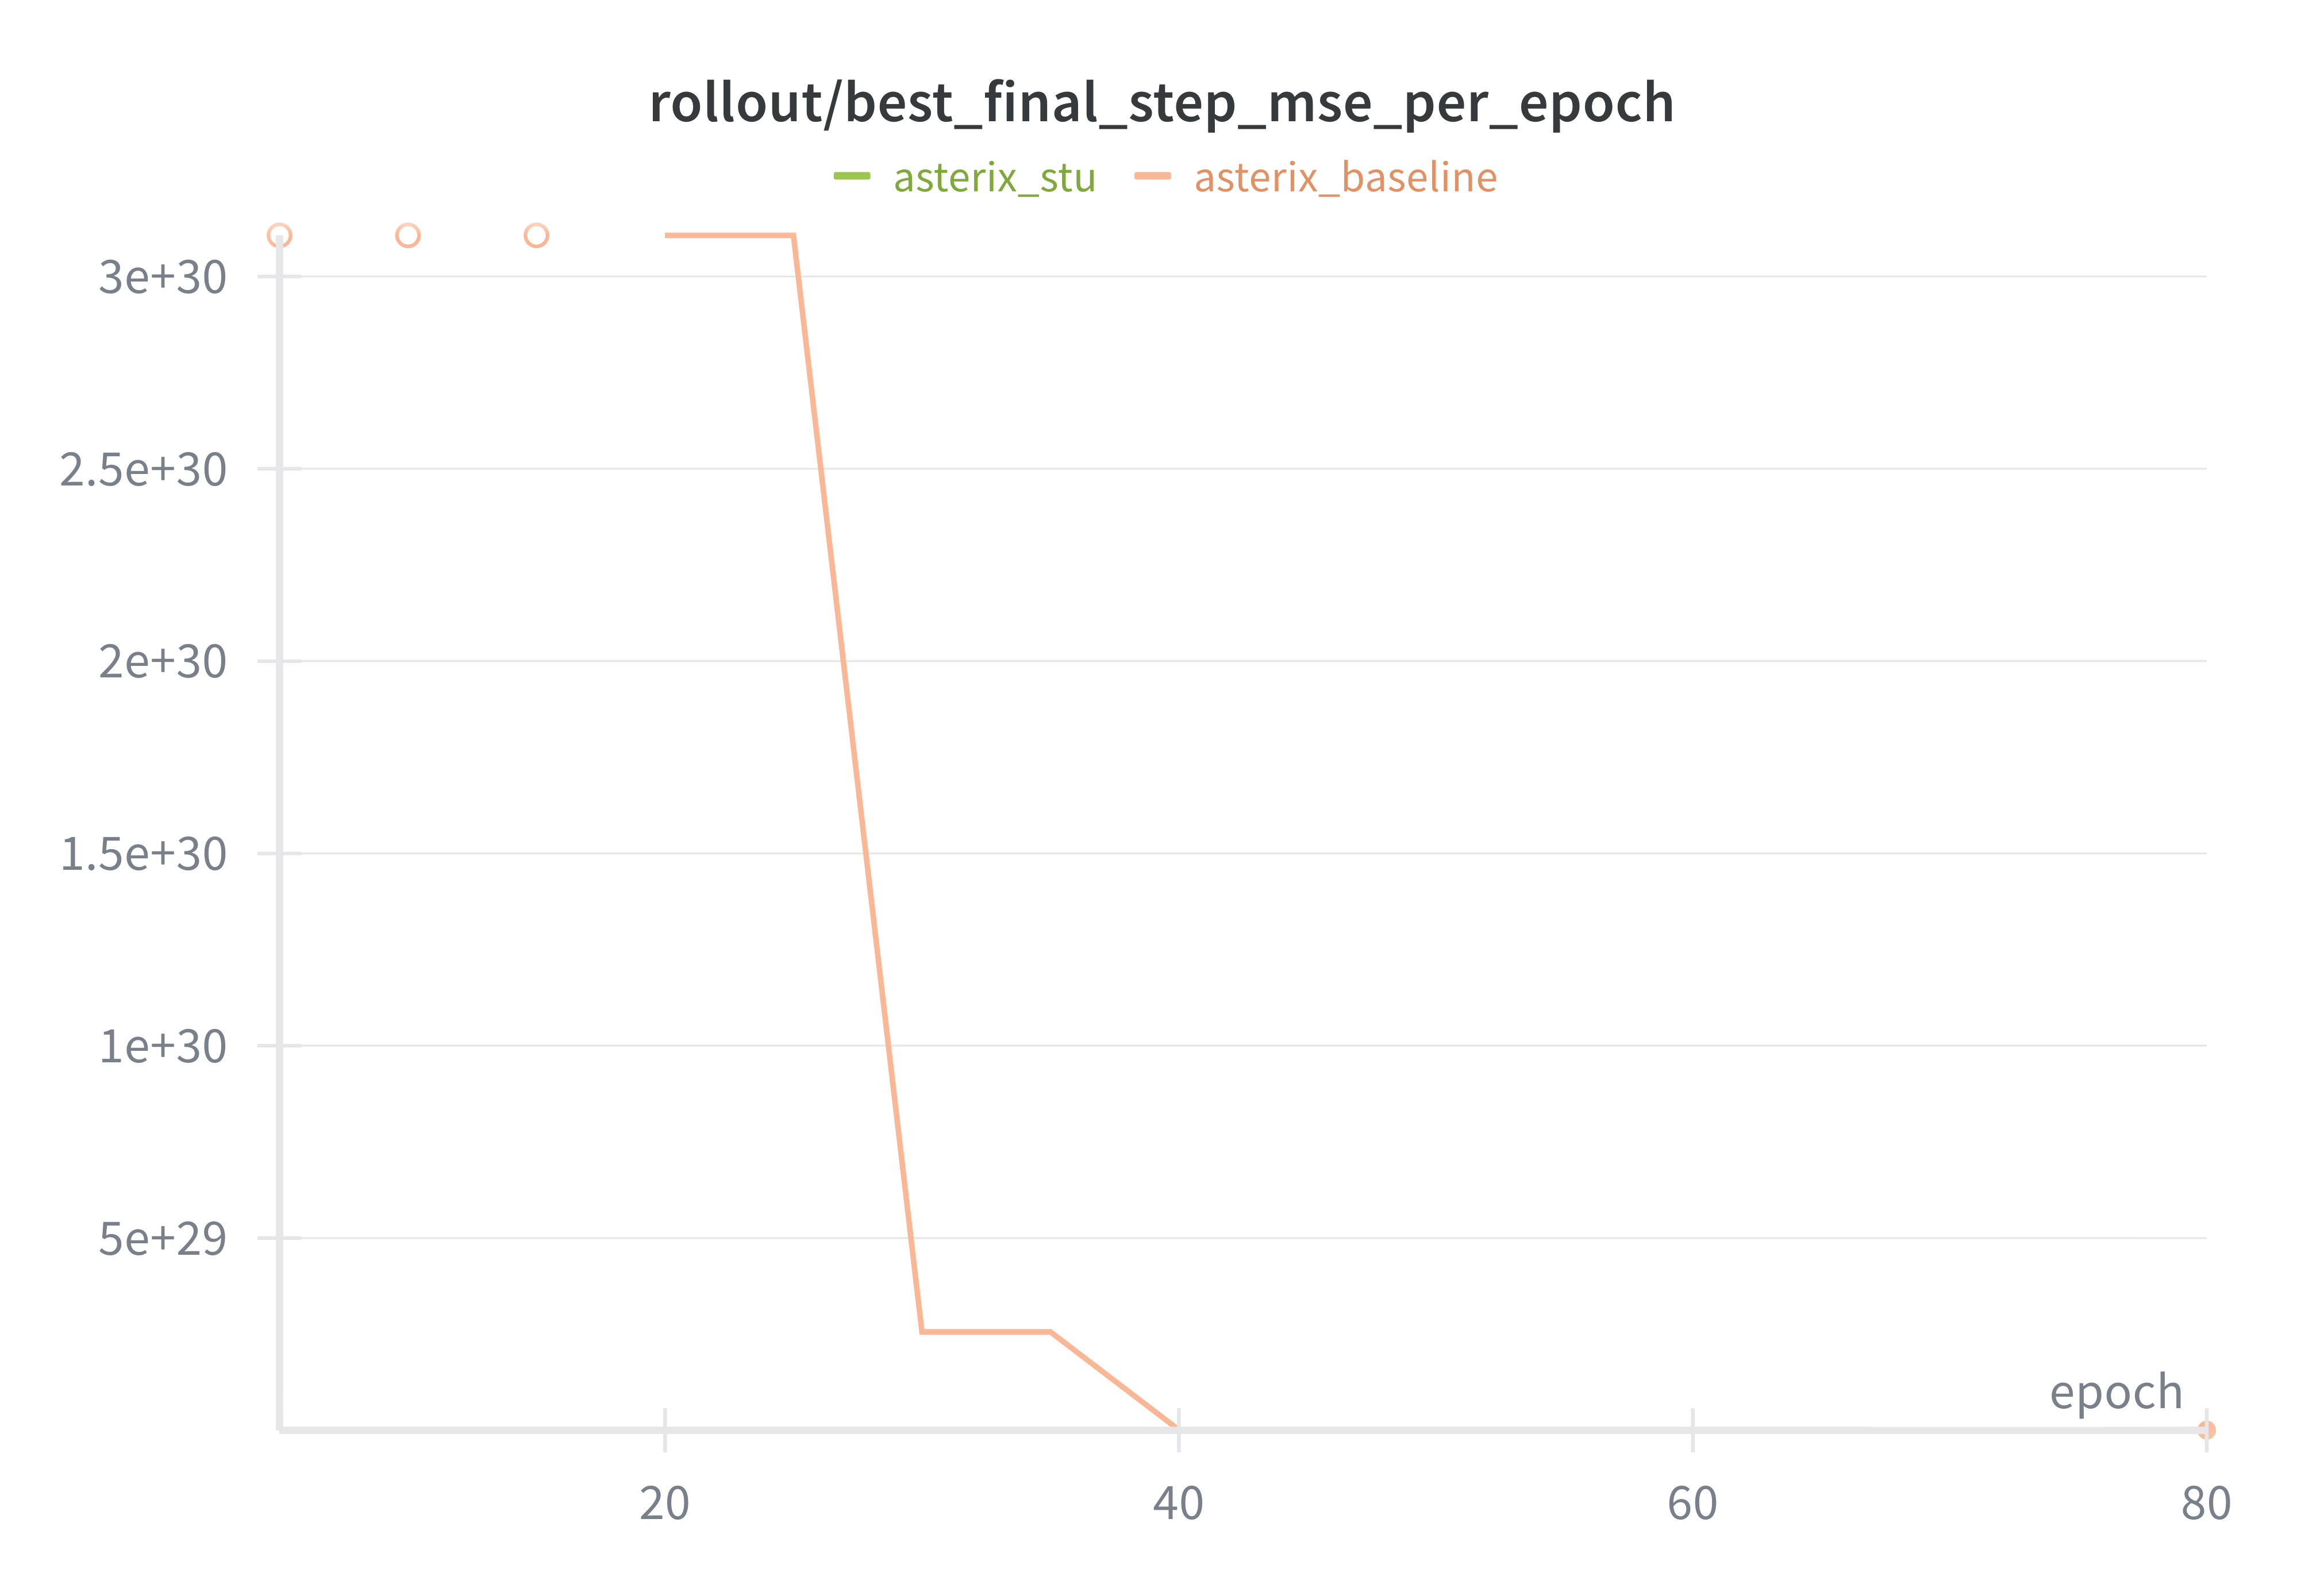
\includegraphics[width=0.9\textwidth]{EXP9_best_final_step_mse_asterix.png}
\caption{Experiment 9: Best final step MSE (step 50 of rollout) over training epochs for Asterix. The Spatial STU dynamics function reaches MSE ${\sim}3.2 \times 10^5$, while the baseline remains at ${\sim}1.25 \times 10^{27}$.}
\label{fig:exp9}
\end{figure*}

To validate that the Pong results were not environment-specific, we repeated the experiment on Atari Asterix, which has a larger action space (9 actions vs.\ 6). The results (Figure~\ref{fig:exp9}) confirm the same pattern. Table~\ref{tab:asterix} shows the MSE at selected rollout steps for both models after training. Notably, the step 50 MSE for Spatial STU does not demonstrate the same bounded behavior as in the Pong environment. This likely correlates with the larger action space in Asterix. However, the gap between STU and the baseline still grows exponentially with rollout length in both Pong and Asterix.

\begin{table}[t]
\centering
\caption{Multi-step rollout MSE: Baseline vs.\ Spatial STU on Asterix.}
\label{tab:asterix}
\begin{tabular}{@{}crrl@{}}
\toprule
Step & Baseline & STU & Ratio \\
\midrule
1  & 0.0009 & 0.0013 & Baseline 1.4$\times$ better \\
5  & 0.013  & 0.005  & STU 2.4$\times$ better \\
10 & 3.4    & 0.025  & STU 137$\times$ better \\
20 & $1.06 \times 10^7$ & 1.3 & STU $8 \times 10^6$ $\times$ better \\
30 & $6.3 \times 10^{13}$ & 125 & STU ${\sim}5 \times 10^{11}$ $\times$ better \\
40 & $2.4 \times 10^{20}$ & 5,529 & STU ${\sim}4 \times 10^{16}$ $\times$ better \\
50 & $1.25 \times 10^{27}$ & 320,708 & STU ${\sim}4 \times 10^{21}$ $\times$ better \\
\bottomrule
\end{tabular}
\end{table}

\subsection{Comparison with Alternative Architectures}

We compared the Spatial STU dynamics function against Spatial Mamba, Spatial Attention, and temporal variants of all three architectures on the Pong dataset.

\textbf{Spatial Mamba} showed partial stability, remaining bounded until approximately 30 steps before diverging. This suggests that Mamba's selective state space mechanism provides some regularization, but less than STU's spectral filtering.

\textbf{Spatial and Temporal Attention} performed comparably to the baseline, showing no meaningful improvement in long-horizon rollout stability.

\textbf{Temporal variants} (Temporal STU, Temporal Mamba, Temporal Attention) all performed similarly to the baseline, with error diverging at long horizons. The temporal modules receive a history of $N$ past states but are trained with only single-step loss, providing no gradient signal to encourage the use of history for long-horizon stability. The history buffer likely becomes wasted information during training, given that we only train with a single-step loss.

\textbf{Spatial-Temporal STU} performed worse than Spatial STU alone, suggesting that the temporal component may interfere with the spatial regularization effect.

These results indicate that the spatial application of spectral filtering is the critical factor, not temporal sequence modeling. The STU's advantage comes specifically from filtering across the $6 \times 6$ latent spatial grid at each step.

\subsection{Experiments 10--14: Online Training with Extended Rollout Length}
\label{sec:online-extended}

Given the offline evidence that Spatial STU excels at long-horizon prediction, we tested whether this advantage could be leveraged in the online EZV2 training loop by increasing the number of recurrent unroll steps from the default of 5 to 10. This parameter controls how many steps the dynamics function is applied autoregressively during training to compute the consistency, value, and policy losses.

\begin{figure*}[t]
\centering
\subfigure[Consistency loss]{
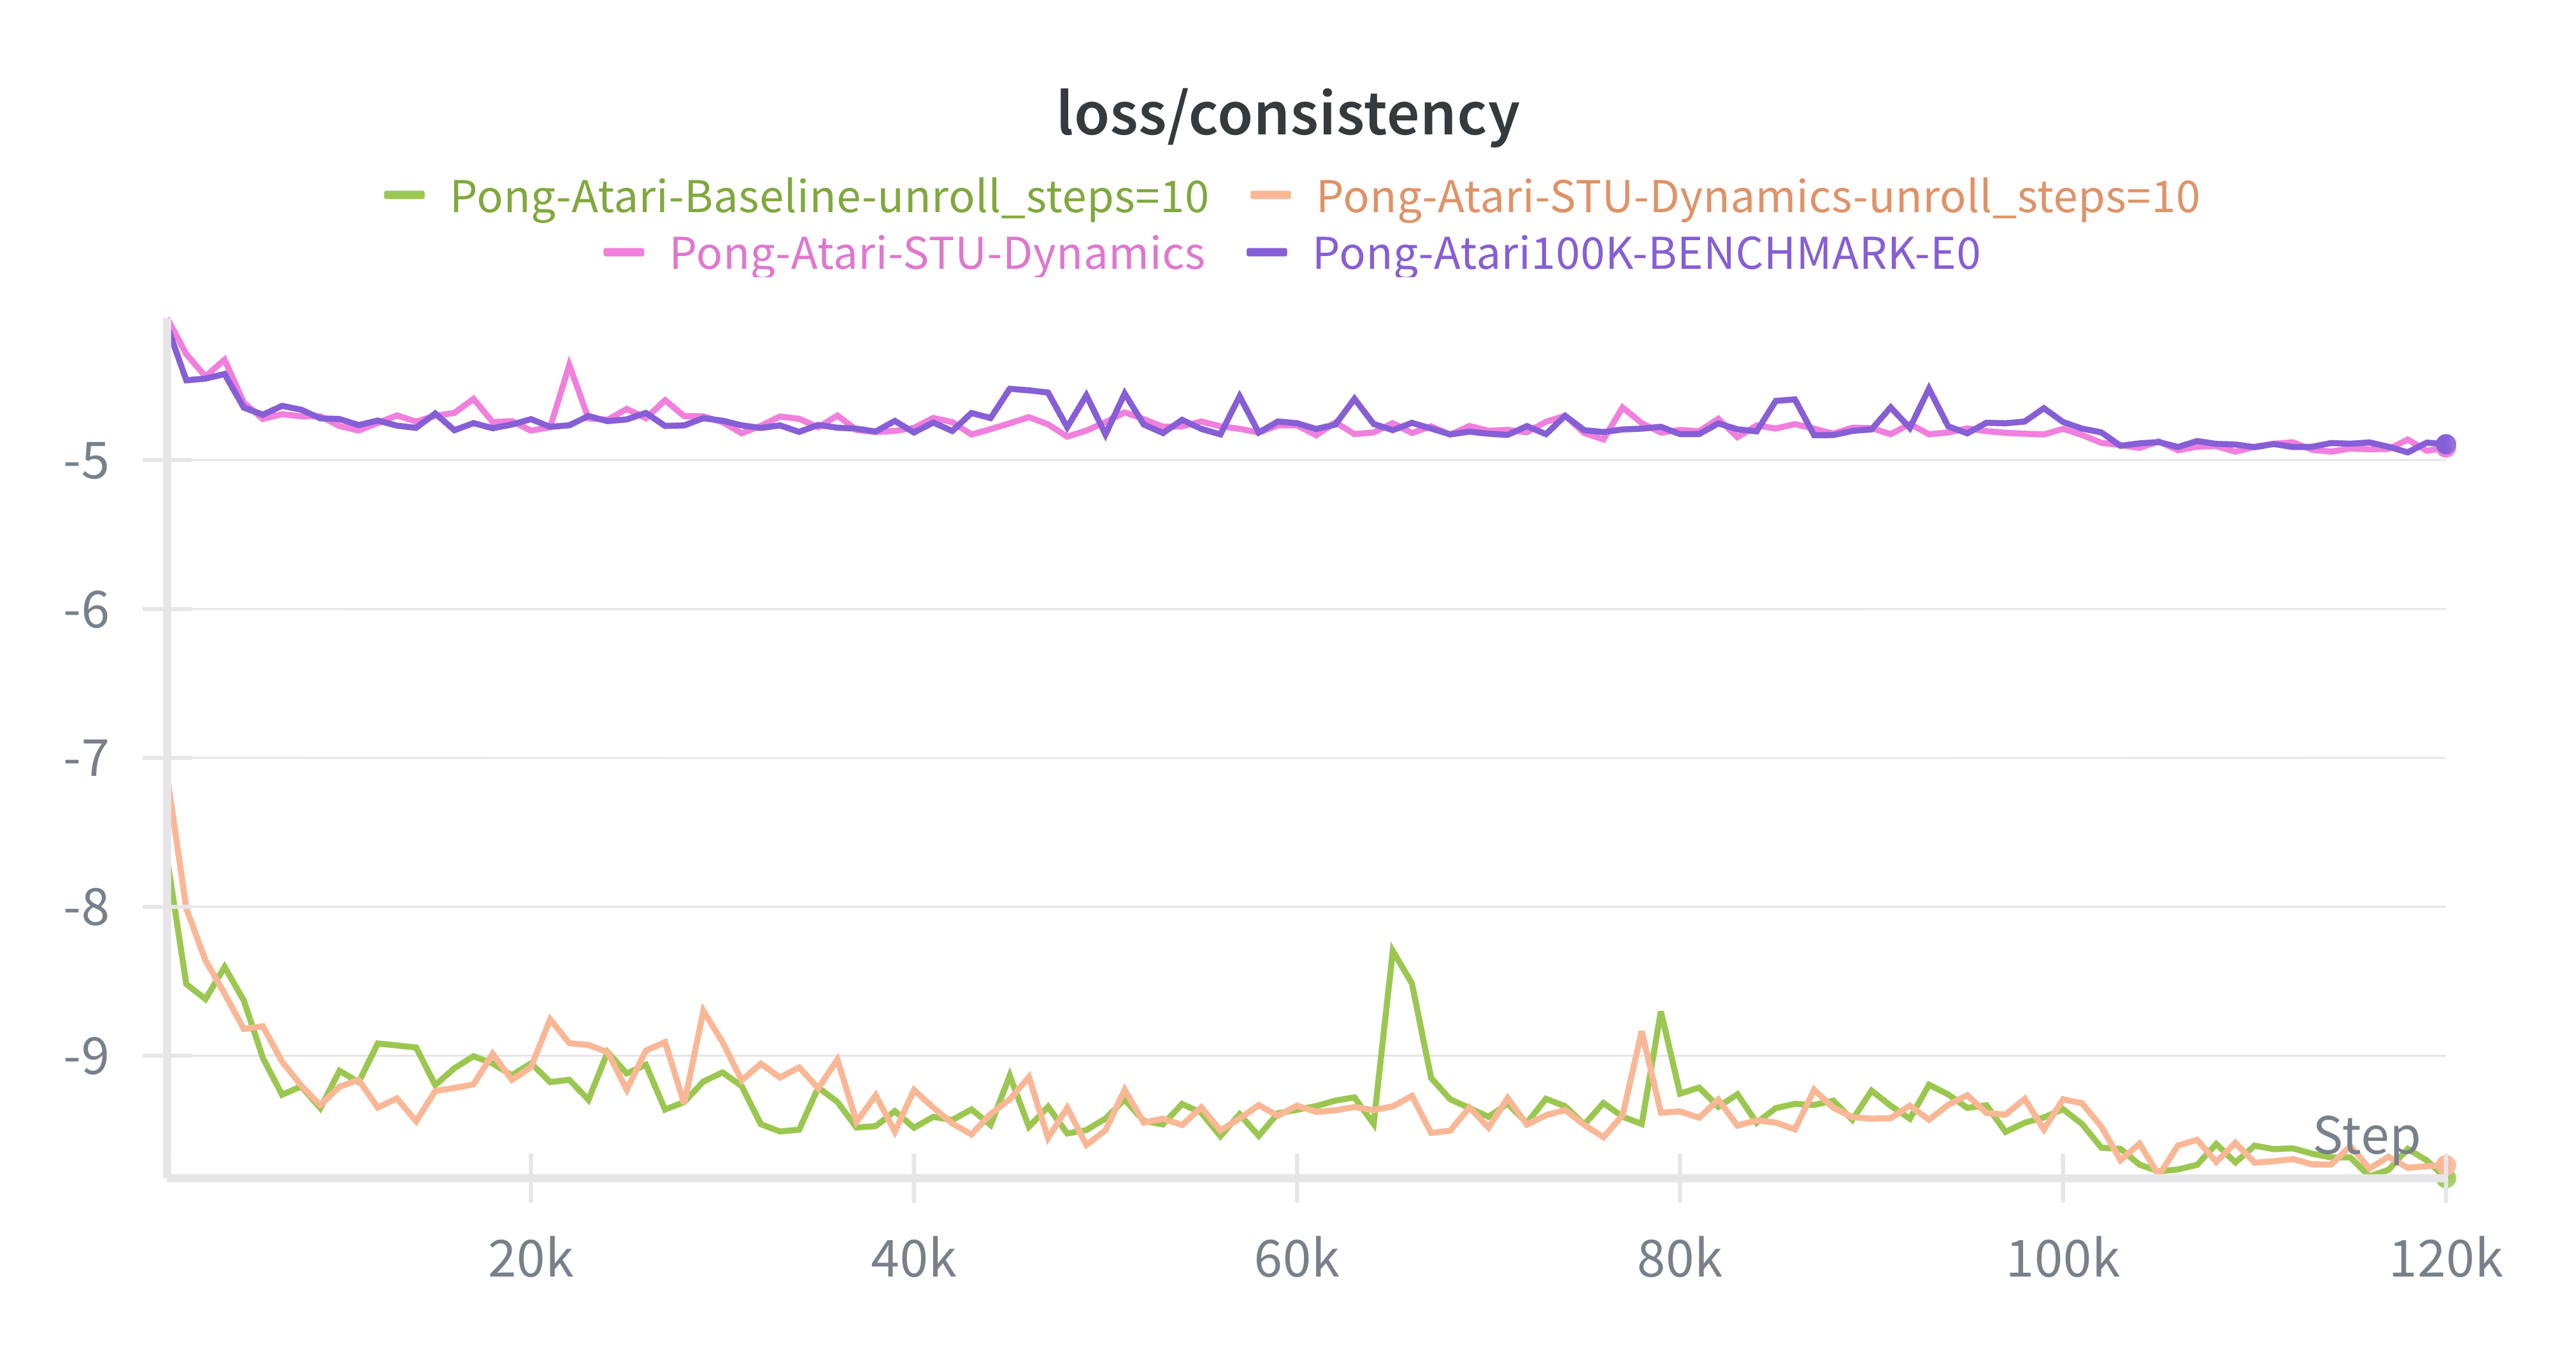
\includegraphics[width=0.45\textwidth]{EXP10_loss_consistency_pong_unroll_steps_10_vs_baseline.png}\label{fig:exp10}}
\subfigure[Policy loss]{
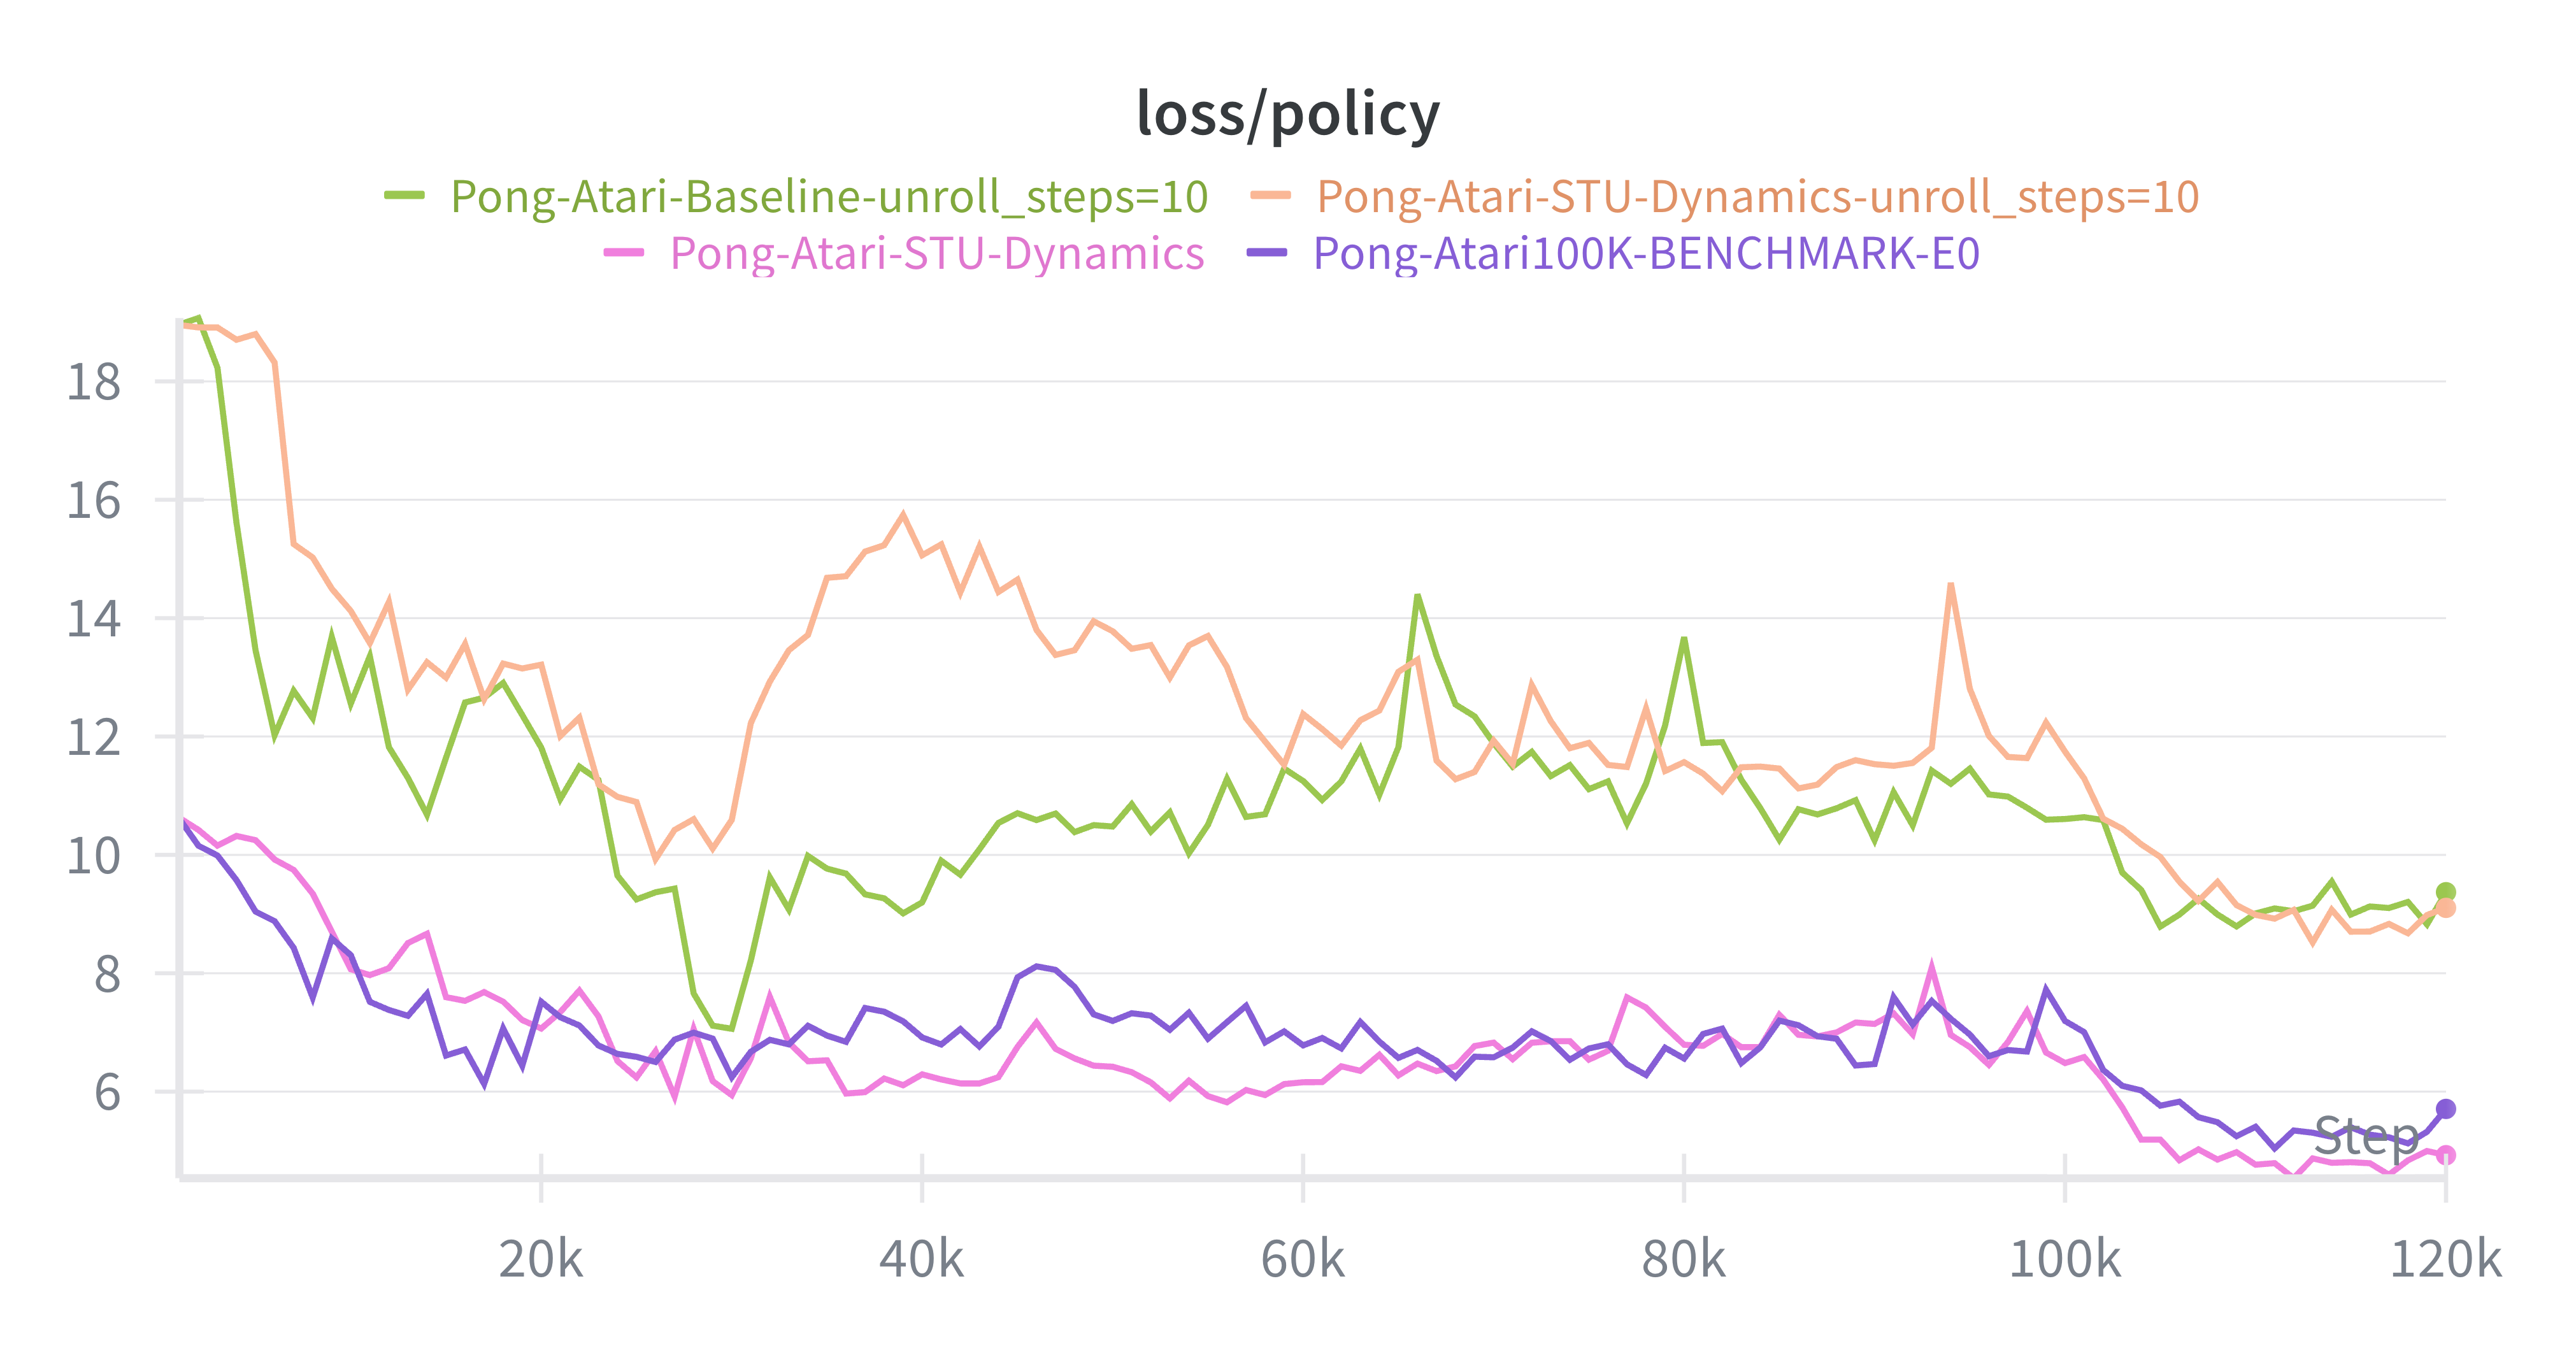
\includegraphics[width=0.45\textwidth]{EXP11_loss_policy_pong_unroll_steps_10_vs_baseline.png}\label{fig:exp11}}

\subfigure[Total loss]{
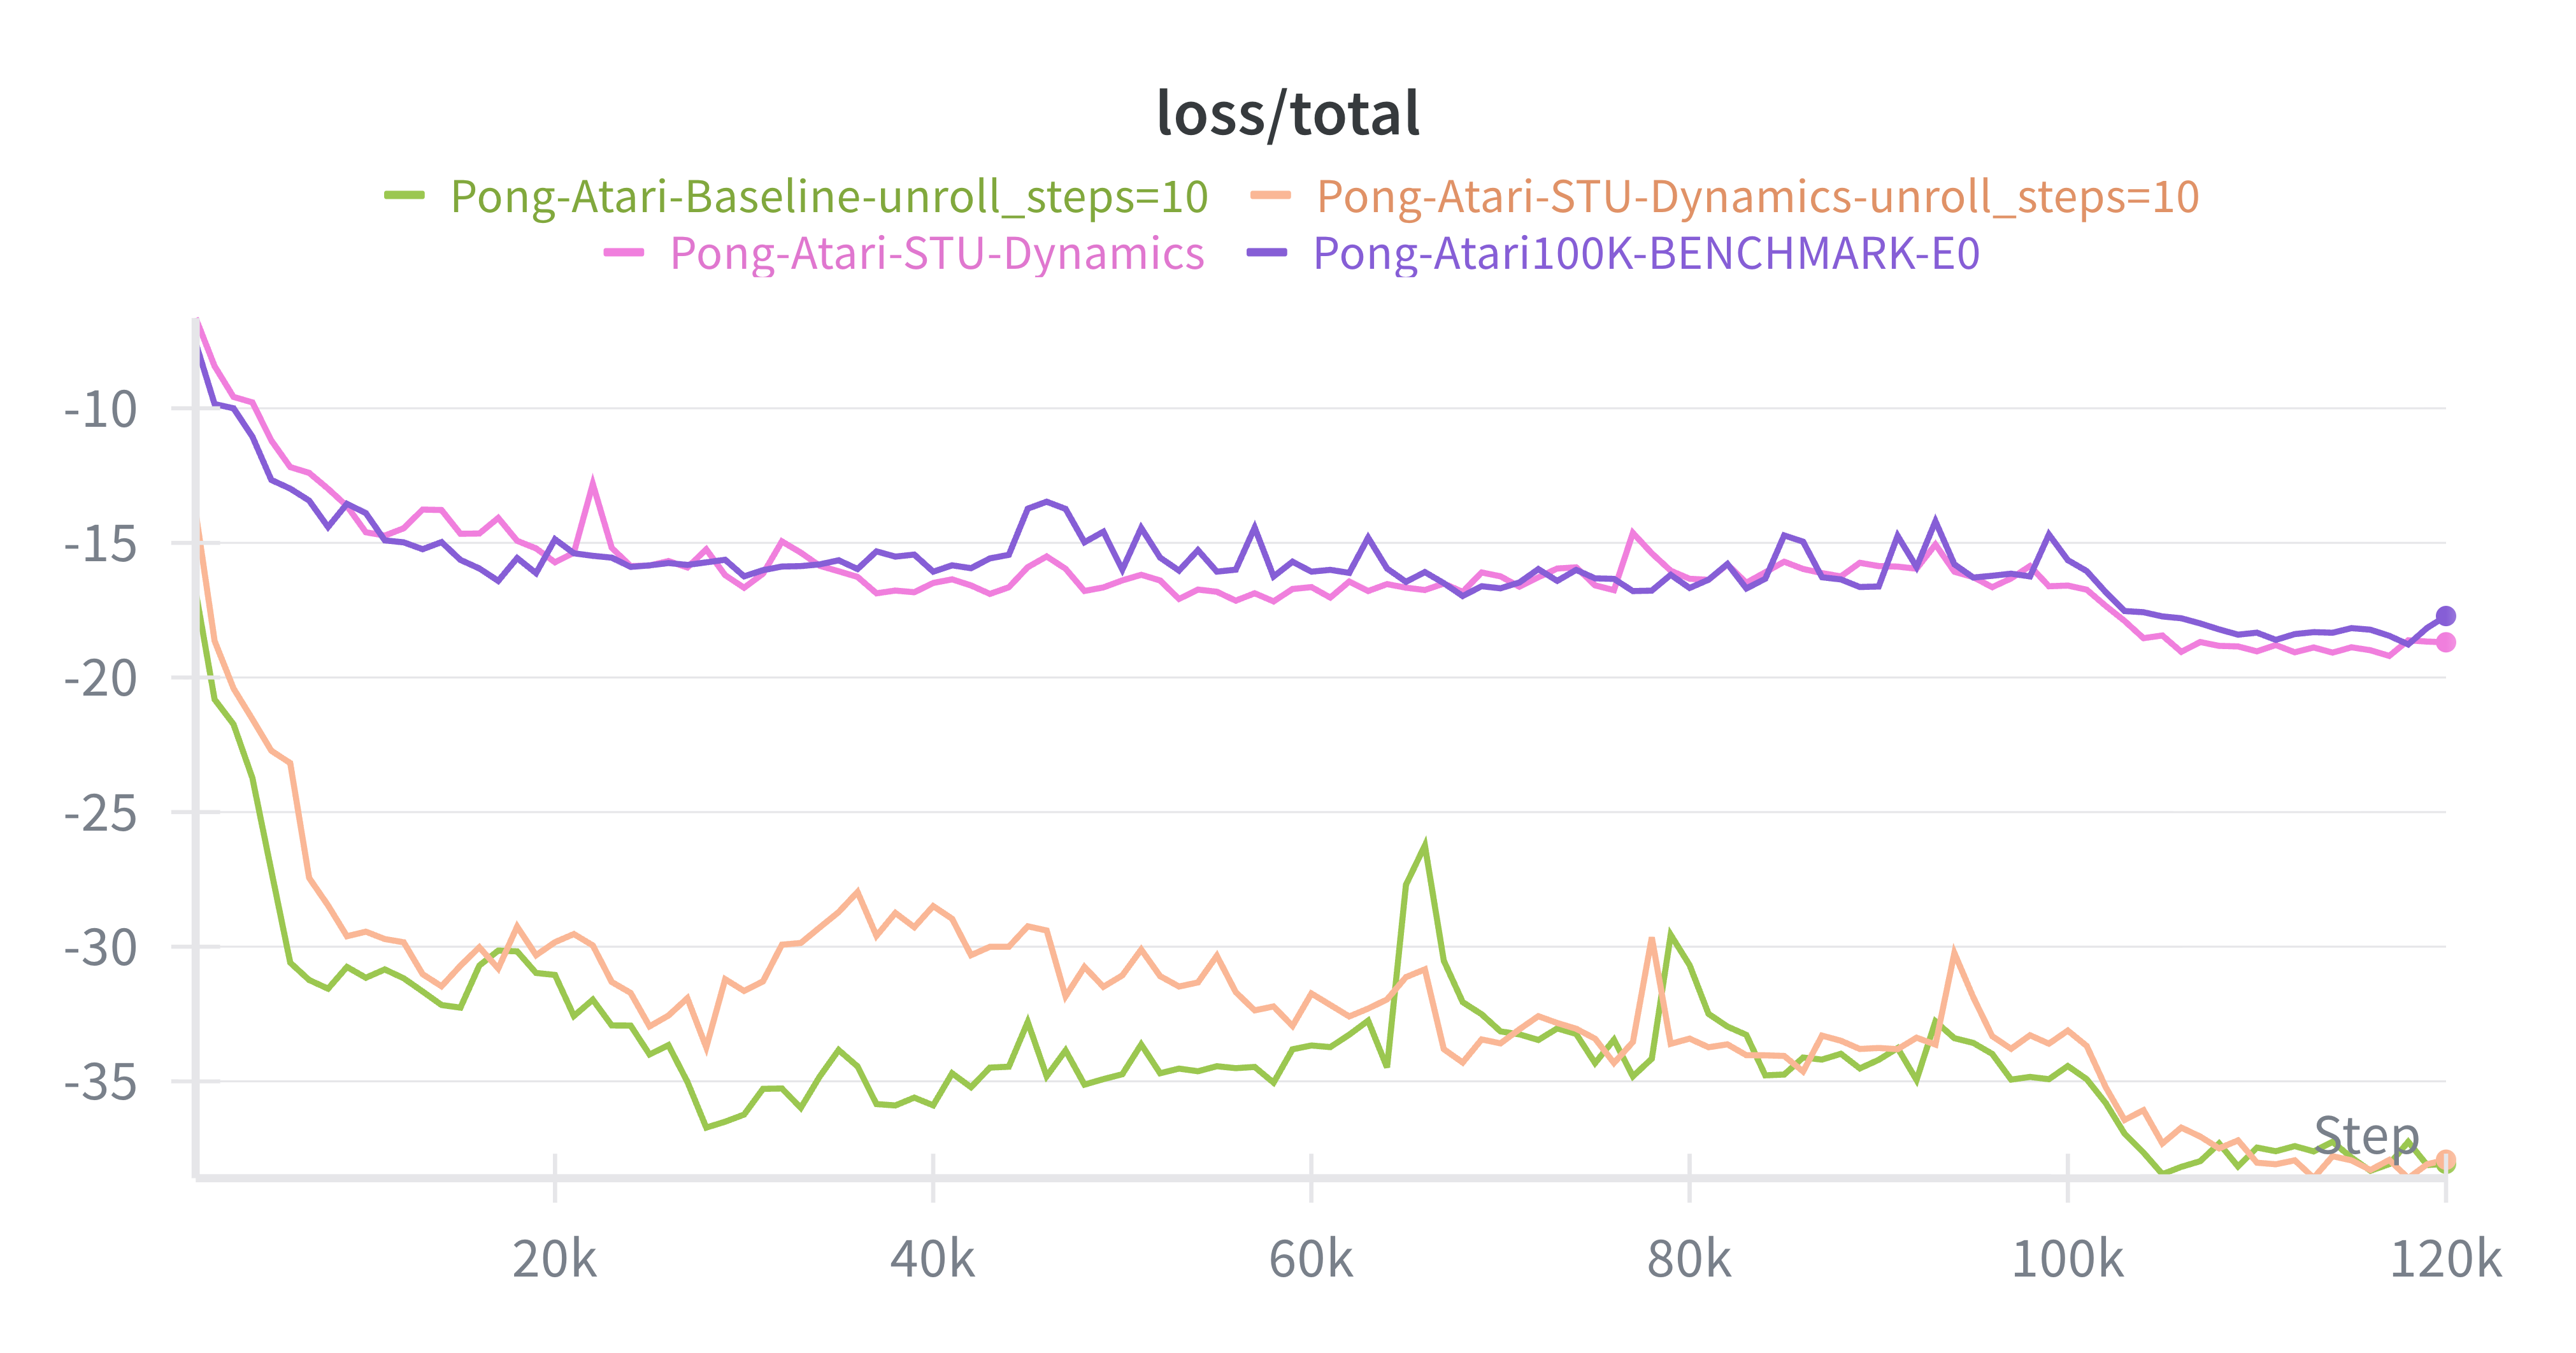
\includegraphics[width=0.45\textwidth]{EXP12_loss_total_pong_unroll_steps_10_vs_baseline.png}\label{fig:exp12}}
\subfigure[Value loss]{
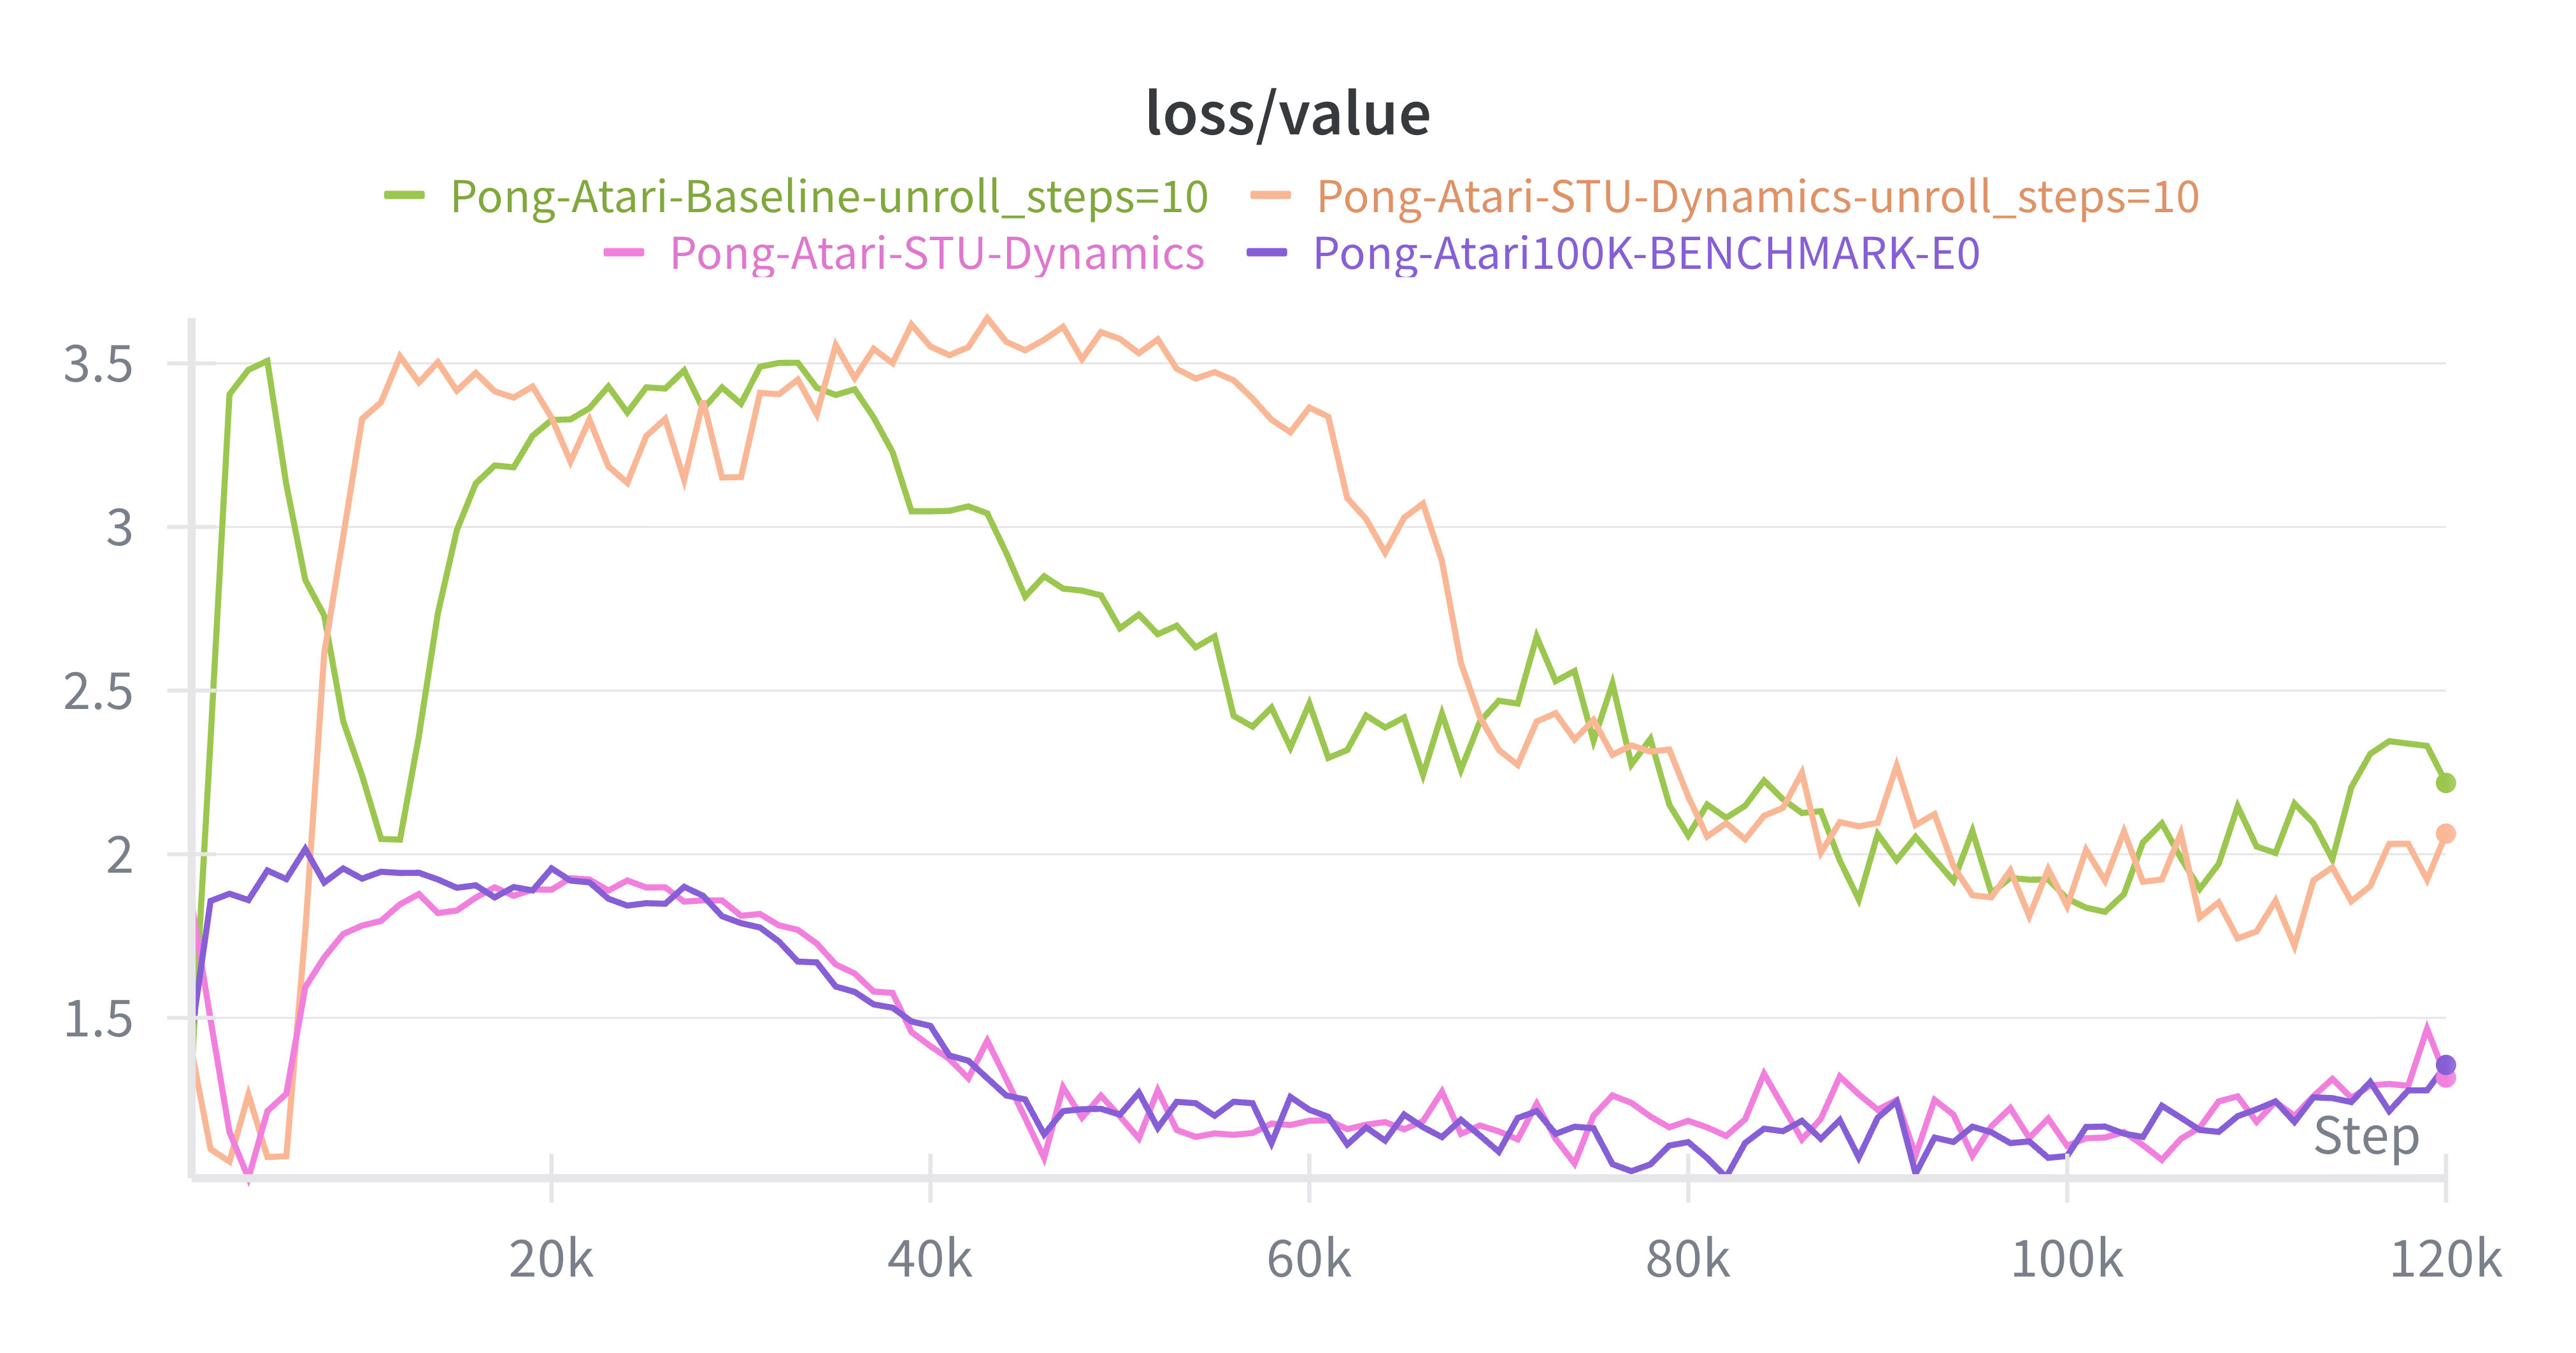
\includegraphics[width=0.45\textwidth]{EXP13_loss_value_pong_unroll_steps_10_vs_baseline.png}\label{fig:exp13}}
\caption{Experiments 10--13: Online training losses comparing STU dynamics and baseline dynamics at rollout lengths 5 and 10 on Pong.}
\label{fig:exp10-13}
\end{figure*}

Figure~\ref{fig:exp10-13} shows four configurations: Spatial STU dynamics (rollout length 5 and 10) and baseline dynamics (rollout length 5 and 10). Two findings emerge:

\begin{enumerate}
    \item Increasing rollout length from 5 to 10 substantially reduces the consistency loss for \emph{both} STU and baseline to a similar extent. This indicates that the baseline dynamics function in EZV2 is already sufficiently accurate for rollout prediction up to 10 steps -- the regime where the baseline begins to become unstable offline is beyond what the online loop tests.

    \item Lower consistency loss does \emph{not} correlate with lower policy or value loss. The training runs with default rollout length 5 achieve better policy and value losses than the rollout length 10 runs.
\end{enumerate}

\begin{figure*}[t]
\centering
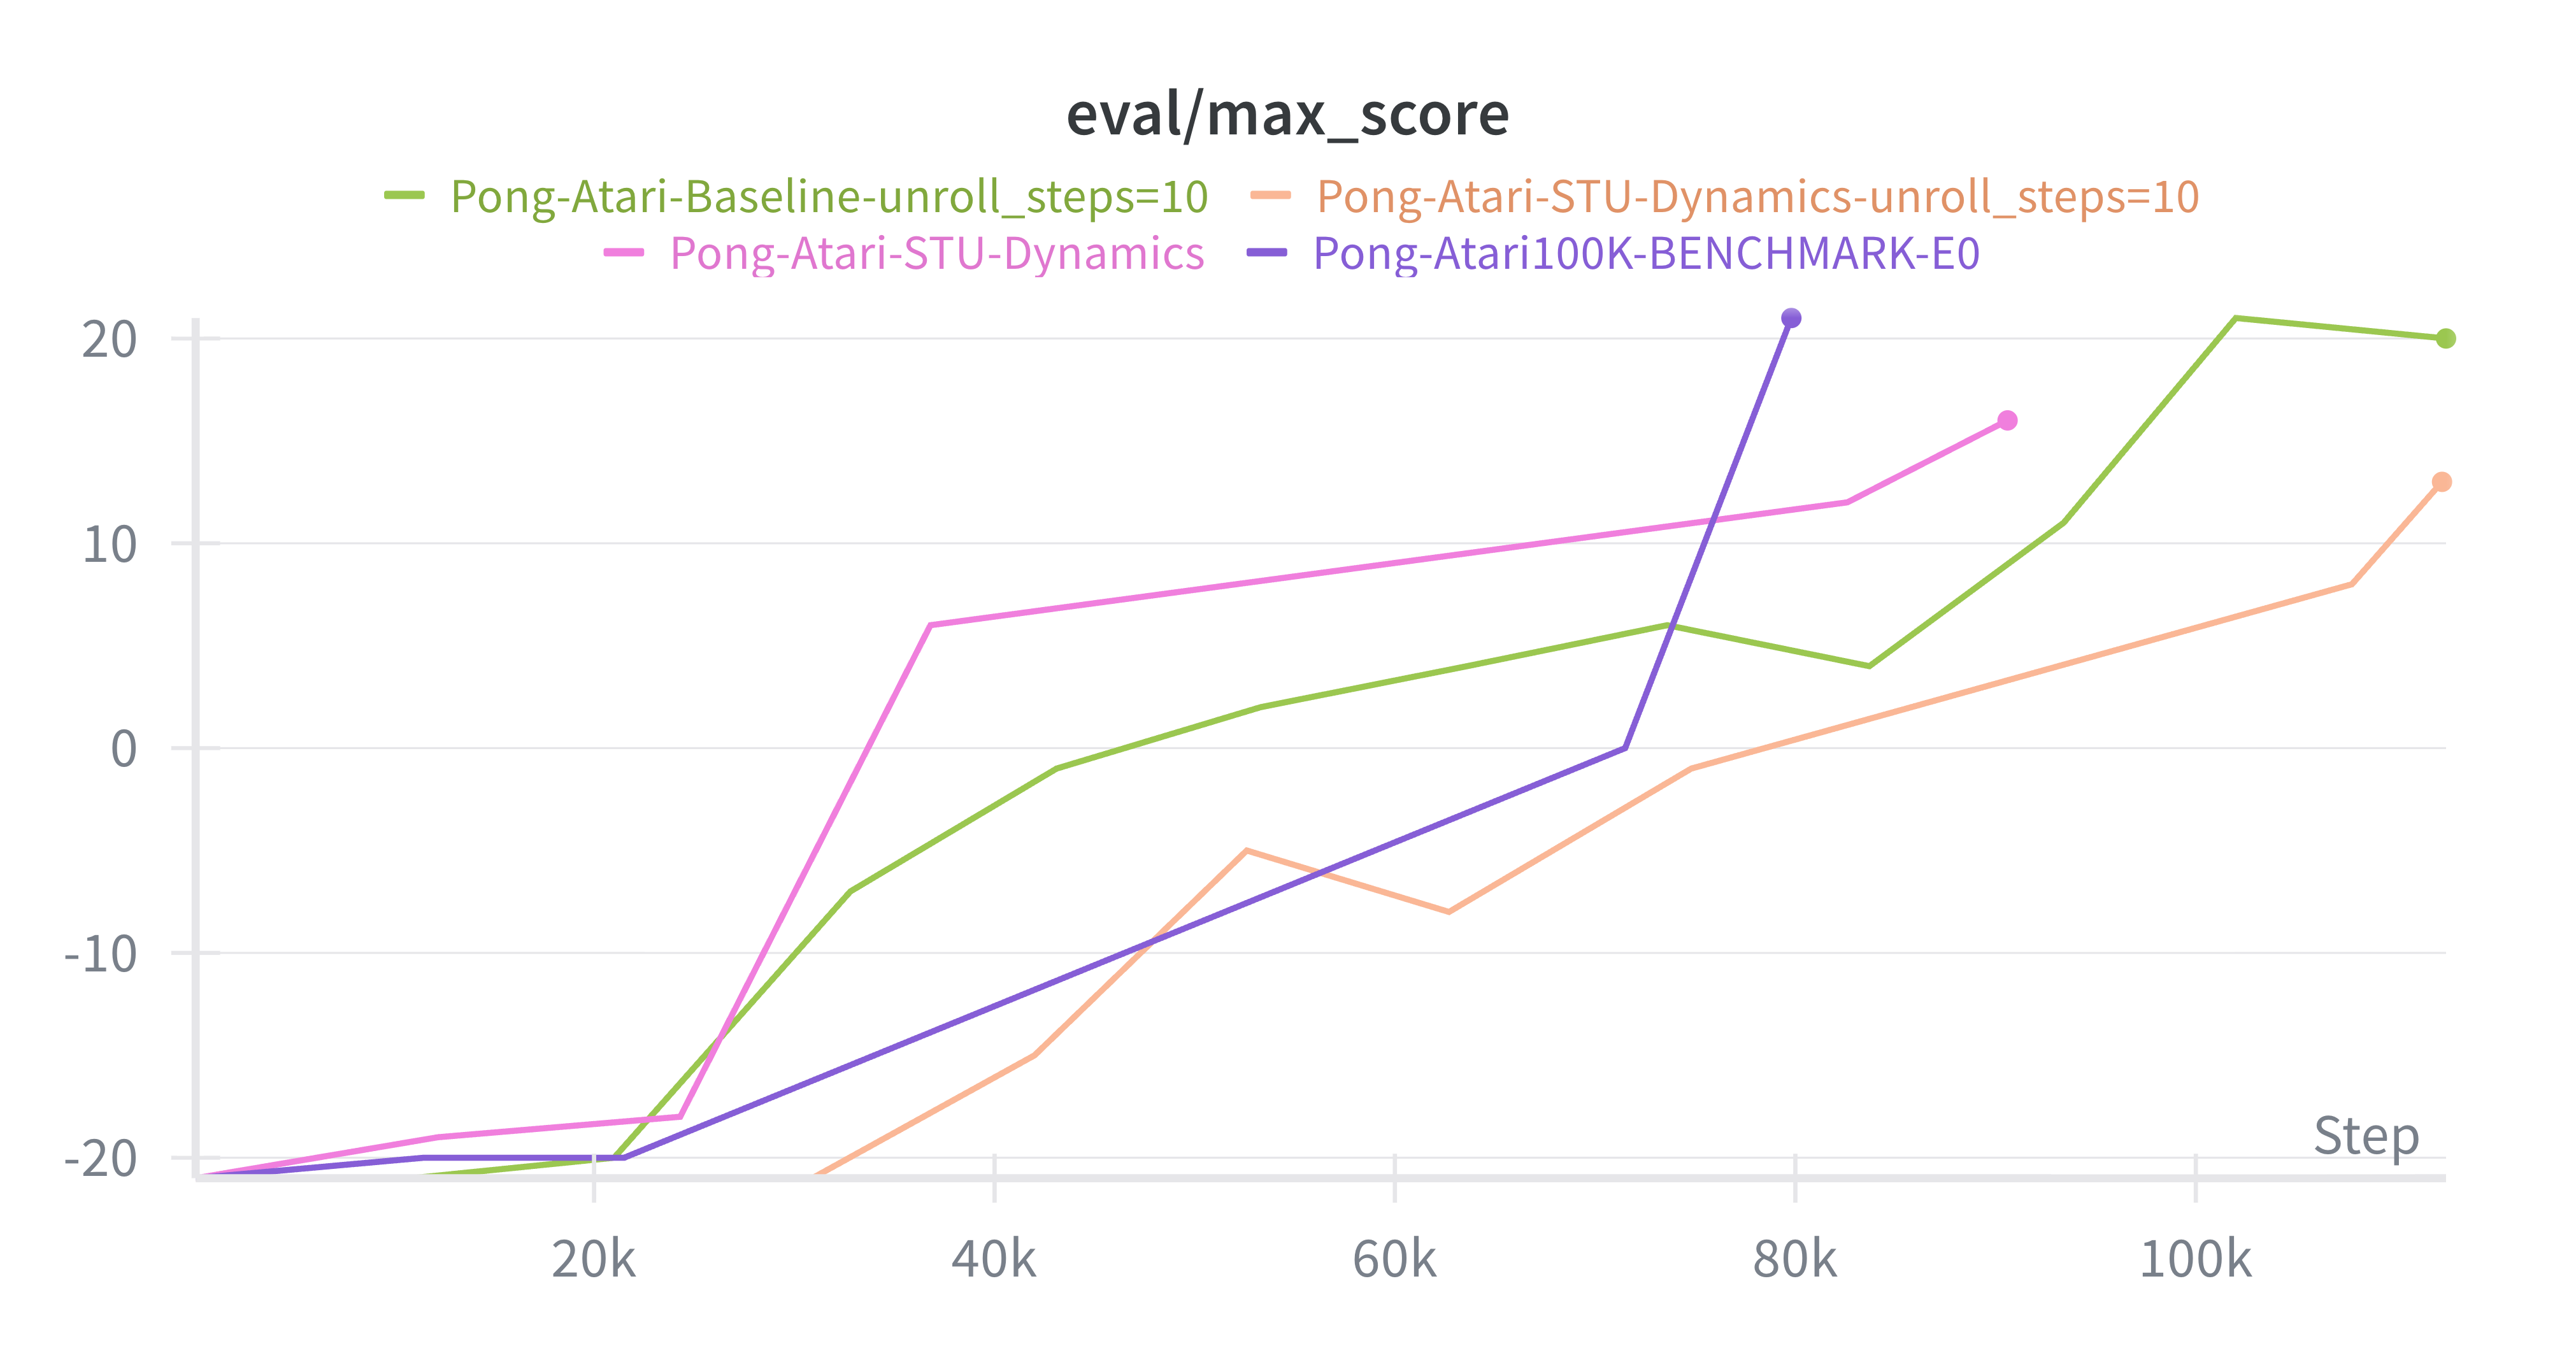
\includegraphics[width=0.9\textwidth]{EXP14_eval_max_score_pong_unroll_steps=10_vs_baseline.png}
\caption{Experiment 14: Maximum evaluation score on Pong comparing rollout lengths 5 and 10.}
\label{fig:exp14}
\end{figure*}

Figure~\ref{fig:exp14} confirms that the maximum evaluation score is achieved more quickly with rollout length 5 than rollout length 10, for both STU and baseline dynamics. This is consistent with the policy/value loss findings.

\section{Analysis}
\label{sec:analysis}

\subsection{Why Does Spatial STU Stabilize Autoregressive Dynamics?}

The key observation is that both the baseline and Spatial STU are trained with identical single-step MSE loss. Neither sees multi-step rollouts during training. Therefore, the stability difference is likely to be an emergent property of the architecture. Spectral filtering in STU produces dynamics that compose better autoregressively, without being explicitly trained to do so. This is a stronger result than if multi-step training were used, because it suggests that the inductive bias of spectral filtering is sufficient to stabilize long-horizon autoregressive generation.

We hypothesize the following mechanism. The eigenvectors of the Hankel matrix $Z$ form an ordered basis from low-frequency to high-frequency patterns (see Figure 1 in~\cite{agarwal2023spectral}). When the STU convolves with the top-$K$ spectral filters ($K=2$ in our best configuration), it projects through a basis that emphasizes smooth, slowly-varying structure and suppresses high-frequency components.

When the dynamics function $G(s_t, a_t)$ is applied autoregressively 50 times, errors compound multiplicatively. The dominant failure mode is high-frequency instability: small per-step errors in sharp or oscillatory components of the latent state get amplified at each step. By filtering through the low-frequency eigenvectors of the Hankel matrix at each step, the STU block effectively projects the output back onto a smooth manifold before it is fed into the next step. High-frequency error modes that would normally grow exponentially are suppressed at every iteration.

This is analogous to why spectral methods in numerical PDE solving are more stable than finite difference methods for long-time integration. Spectral methods represent the solution in a smooth basis (Fourier, Chebyshev) that naturally damps high-frequency numerical artifacts.

Several of our experimental observations support this hypothesis:
\begin{itemize}
    \item Increasing $K$ (number of filters) beyond 2 hurts performance, because higher-frequency modes are retained
    \item Spatial application (filtering across the $6 \times 6$ grid) is effective, while temporal application is not, consistent with errors manifesting as spatially incoherent noise
    \item The effect is architecture-specific: Mamba provides only partial stability (to ${\sim}30$ steps) while attention performs similarly to the baseline
\end{itemize}

\subsection{Why Doesn't This Help Online Atari?}

The offline results show that the baseline dynamics function becomes unstable around ${\sim}10$--20 steps. However, EZV2 uses a default of 5 recurrent unroll steps during training, and in this regime the baseline and STU dynamics functions are roughly equivalent. The STU's advantage is in predicting steps 20--50 accurately, but leveraging this would require:

\begin{enumerate}
    \item Setting the unroll steps to 20 or more, which is computationally prohibitive (estimated $>$150 GPU-hours for Atari with 50 unroll steps, compared to ${\sim}$15 hours with the default of 5)
    \item Demonstrating that longer rollouts actually improve downstream policy quality. However, our initial experiments suggest that lower consistency loss resulting from longer rollouts did not translate to lower policy/value loss or higher evaluation scores
\end{enumerate}

\textbf{This may imply that in the specific application of solving Atari games via EZV2, spectral filtering's utility for long-horizon prediction stability in world models addresses a problem that is not useful to solve.}

\section{Next Steps}
\label{sec:next-steps}

\begin{enumerate}
    \item \textbf{Scale to all 26 Atari games}: Train expert models and collect offline datasets for the remaining 24 games tested in the EZV2 paper. Validate whether the Spatial STU's long-horizon stability advantage holds across diverse environments.

    \item \textbf{Alternative architectures}: Evaluate S4~\cite{gu2022efficiently} and S4D as spatial mixers, and investigate whether the Mamba implementation can be improved to match STU's stability properties.

    \item \textbf{Continuous control environments}: Test Spatial STU on the continuous control environments from the EZV2 paper, where longer planning horizons may be more beneficial.

    \item \textbf{Extended rollout horizons}: Test rollout lengths beyond 50 steps for each game. Determine whether the Spatial STU's MSE error remains bounded at longer horizons.

    \item \textbf{Theoretical analysis}: Develop a formal understanding of why spectral filtering produces an inductive bias that prevents error compounding in autoregressive dynamics prediction.

    \item \textbf{Multi-step training loss}: Evaluate whether training with a multi-step rollout loss (predicting $k$ steps ahead autoregressively, with loss on each) amplifies the STU advantage or enables the baseline to learn comparable stability.
\end{enumerate}

\section{Conclusion}
\label{sec:conclusion}

This report documents progress toward building world models for reinforcement learning using Spectral Transform Units. Through a combination of online experiments within the EZV2 framework and an offline dynamics training methodology, we have identified an emergent property of spatial spectral filtering: when applied as a spatial mixer over the latent state grid, STU produces dynamics functions that are inherently stable over 50-step autoregressive rollouts, even when trained only with single-step loss. This effect is significantly stronger than comparable modifications using Mamba or self-attention, and is achieved with fewer parameters than the baseline EZV2 dynamics function implementation.

However, we also claim that this capability may not translate to improved online Atari performance, as the baseline dynamics function is sufficient for the short rollout lengths used in practice. The most notable contribution here may be the demonstration that spectral filtering produces an inductive bias toward composable dynamics, which could prove valuable in domains other than Atari that require longer planning horizons.

\bibliographystyle{IEEEtran}
\bibliography{references}

\end{document}
